\documentclass[12pt,a4paper]{article}
  \usepackage[toc,page]{appendix}
  \usepackage{longtable}
  \usepackage{listings} 
  \usepackage{verbatim}
  \usepackage{graphicx}
  \usepackage{tabularx}
  \usepackage{subfig}
  \usepackage{float}
  \usepackage{csvsimple}
  \begin{document}
    \begin{titlepage}
      \centering
      {\scshape\LARGE Goldsmiths, University of London \par}
      \vspace{1cm}
      {\scshape\Large Software project proposal\par}
      \vspace{1.5cm}
      {\huge\bfseries iLost\par}
      \vspace{2cm}
      {\Large\itshape 
        Ahmed, Muhammad\\
        Chowdhury, Thairan\\
        Davies Minta, Dylan\\     
        Fakrul, Mahmudul\\    
        Farkhani, Hussein\\ 
        Jheng-Hao, Lin\\
        Pecorella, Mariano\\ \par}
      \vfill
      supervised by\par
      \textsc{Tim Blackwell} 
      \vfill
      % Bottom of the page
      {\large \today \par}
    \end{titlepage}

    \tableofcontents
    \newpage
    

    \section{User Need Overview \& Concept Introduction}
      \subsection{Subsection}
        \paragraph{}
          We began our process of conceptual development by questioning fellow students about some of the everyday issues they encounter to aid us in coming up with an idea capable of mitigating a specific need. During these conversations, the group found that losing personal belongings in both private and public places was a common occurrence. According to research from Mozy, the average value of a lost item is £131.67; the average person irretrievably loses £71.55 of goods each year. As a result of the average person losing over £60 worth of possessions each year; billions are being lost.\cite{LostAndFound} To satisfy the needs of our users, we focused on finding a way to circumvent the loss of items; we determined that developing an item loss prevention app would be appropriate.
      \subsection{Concept Introduction}
        \paragraph{}
          Our app's original intention was to inform the owner that they're about to leave a belonging behind by sending a notification to their phone upon reaching a certain distance away from the item. To facilitate this concept, we needed a means for the app to communicate with the lost possession and concluded that a tracking device of our own would be necessary. We wanted to ensure that the tracking device was discreet; hence our group set its initial focus on Bluetooth stickers. Bluetooth stickers seemed to be a natural choice because they’re lightweight, making them easy to carry around. Additionally, we thought it was the appropriate choice for our project due to how inexpensive these items can be, as well as low power consumption and high accuracy. A Bluetooth tracking device is rendered useless by a dead battery and numerous other potential complications. To counteract this, we adopted a hybrid approach, utilising Bluetooth in conjunction with cellular data, Wi-Fi and a server, enabling logging over greater distances.

    \section{Data Gathering and Requirements}
      \paragraph{}
        According to our research, the external stakeholders include the potential users. As the developers of this idea, we are the internal stakeholders. Our project is designed to aid users. Therefore, our aim as internal stakeholders is to address the concerns of the external stakeholders.[1] We carried out a user investigation using SurveyMonkey, to garner a better understanding of our potential clientele. We gained knowledge that 44\% of the interviewees would be very likely to buy the product if it’s available today. Analysing the data trends of the 54 responses we received informed us that 70\% of the interviewees had a positive reaction to the concept. The remaining percentage was concerned about our concept’s similarity to other existing products; [2] the concerns that were raised made it a requirement for us to find ways to distinguish our project from others.
      \paragraph{}
        Our team gathered data in many ways, helping us meet the stakeholder's requirement of differentiating ourselves. We used the market research, motivated by the survey interviewee’s concerns, to provide ways in which we can diversify our idea from existing products or solve their shortcomings. Comparing the pros and cons of similar concepts allows us to combine the best of each. Product reviews uncovered a flaw in existing products; users deplore the fact that they aren’t notified if an item is about to exceed the tracker's range.[3] This improvement users are shown to be longing for[3] is also an integral part of our original idea and this distinguishes us from what exists. This research influenced our decision to utilise GPS triangulation, which is also nonexistent in current products and expands on the general concept.
    
    \section{Functional Specification}
      \paragraph{}
        Our product has the ability to prevent the loss of personal belongings as well as, retrieve lost belongings. How does it do that?
      \paragraph{}
        We will accomplish this through a hybrid approach, utilizing small computers and the precision of short range wireless technology as well as long range wireless technology (essentially unlimited range). Given different scenarios, these technologies will alternately adapt according to the user’s needs. Through the medium of software application, the user will be able to interact with the tracker on the tagged item. Here is how the application works: 
      \begin{enumerate}  
        \item The application will allow sending requests to the server in order to create a new account, to store a new user’s data in the database. It will also consent: •	
        \begin{itemize}  
          \item updating account details
          \item retrieve existing users’ data from the server once the application has acknowledged sign in details.
        \end{itemize}
        \item The customer will have to then register item/s of interest that needs to be tracked. This can be done by selecting from an existing items list of items as well as adding a new item label to be tracked.
      \end{enumerate}
      \paragraph{}
        In a normal scenario:
        \begin{enumerate}  
          \item The smartphone will be tracking the user’s position.
          \item The application on the phone will frequently request the labelled items’ location tagged by tracker utilizing the short range wireless communication technology by default.
          \item In the event of the application not detecting signals from short range wireless technology in the tracker. This will trigger the application to send out a notification to the smartphone, warning the user that the item is not in their neighbouring.
          \item In this case the item is out of the user’s range, so the user can head back to the location to recover the item.
          \item The customer can also choose to stop the notification temporarily and retrieve the item in a later time.
          \item Once the user is back within the range of receiving signals from the tracker to the application, the notification will then permanently stop.
          \item The incident will then be recorded and stored on smartphones’ database as lost history with the marked location.
          \item On the other hand, long range wireless technology mounted on the tracker comes in play when an object needs to be recovered or tracked once it is out of the short reading range.
        \end{enumerate}  
      \paragraph{}
      In this case the consumer can utilize the application to interact with the tracker, and switch to the long range wireless technology for it to locate itself displaying the position of the tagged item. At this stage, the location of the item has a vague accuracy range, approximately around 40 metres. However, as the user progresses towards the tagged item the application will notify the long range wireless technology server to switch on the short range wireless technology for greater accuracy of positioning range, roughly of 3 metres distance.

    \section{Ethical Audits}
      \paragraph{}
        Ethical audits are a set of rules and regulations that a business is considered to follow. It is a platform in which, priorities different factors and signifies right from wrong. Ethical audits can be both internal and external to the business. The five sectors that are usually looked at under ethical audits are data protection/customer data/privacy, health and safety, labour, environmental ethics and business ethics. Labour however can fall both under environmental or business ethics.
      \paragraph{}    
        One question that is likely to be asked right off the bat by potential customers is regarding their personal data. As it is a device that not only alerts the user that they have left a product behind, it also allows the user to locate their missing product/s. Our data protection will serve a disclaimer, the application will have a “Terms of Use” script which tells the user that their data is safe as iLost will only need location data. Now, this might raise further questions, to put any disputes to bed. The data that iLost will use is longitude and latitude just to track the lost property/properties, meaning all other customer data will not be affected. To still have a strong backing, we will make the device as safe to the customers use as possible. Privacy therefore should not be a issue for the user. All the data that we collect, will be stored with ICO (Information Commissioners Office) which is already an established company. iLost will also give the freedom to users to delete any data whenever they want. 

    \section{Design}
        We have six basic use cases which contain five use case actors. These use cases cover all the services our service could provide for the users, which enable us to develop the use case diagram, sequence diagram and activity diagram.
        
        \paragraph{}
          \begin{table}[H]
            \centering
            \resizebox{\textwidth}{!}{
              \begin{tabular}{cl}
                \hline
                  Name & Description \\
                \hline
                  User & The user who uses our service. \\
                  App & The iLost mobile application that User interacts with. \\
                  Server & Hologram Cloud APIs, which provides the geolocation of the Tracker. \\
                  Tracker & Physical tracker attaching to the user's item(s), a raspberry pi and a GPS module are built-in. \\
                  Item & User's personal belonging which is desired to be tracked. \\
                \hline
              \end{tabular}
            }
            \caption{Use case actors} 
          \end{table} 

          \begin{table}[H]
            \centering
            \resizebox{\textwidth}{!}{
              \begin{tabular}{clcl}
                \hline
                  Use Case ID & Use Case Name  & Primary Actor  & Description \\ 
                \hline
                  1 & Log Tracker &  User &  User logs the Tracker into App. \\
                  2 & Monitor Tracker &  App &  App listens to the signal of Tracker. \\
                  3 & Track Item &  User &  User uses App to track their item. \\
                  4 & Send position data &  Tracker &  Tracker sends position data. \\
                  5 & Register account &  User &  User register a new account in App. \\
                  6 &  Login account &  User &  User login to account in App \\
                \hline
              \end{tabular}
            }
            \caption{Use case index} 
          \end{table} 
        
        \paragraph{}
          Please find the details of each use case flow in Appendix \ref{appendix:use-case-flow}.
          
        \subsection{Use cases diagram}
          \begin{figure}[H]
            \centering
            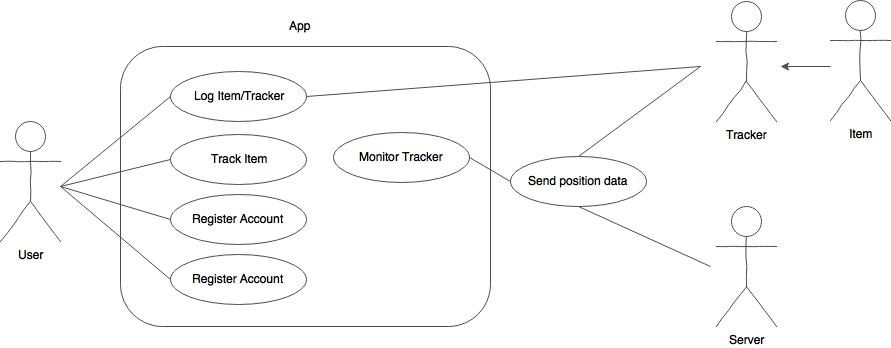
\includegraphics[width=1\textwidth]{assets/5-use-case-diagram.jpg}
            \caption{Use case diagram}
            \label{fig:Use case diagram}
          \end{figure}
          The use case diagram visualises the relationship between these five actors and the use cases.

        \subsection{Sequence Diagram}
          \begin{figure}[H]
            \centering
            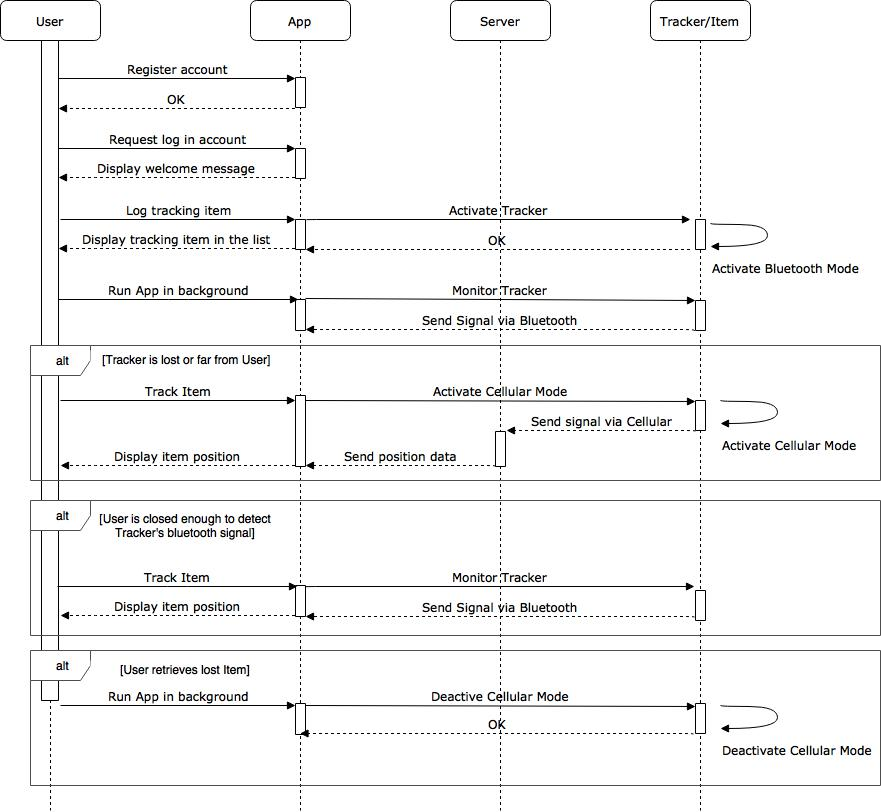
\includegraphics[width=1\textwidth]{assets/5-sequence-diagram.jpg}
            \caption{Sequence diagram}
            \label{fig:Sequence diagram}
          \end{figure}
          The sequence diagram demonstrates the relationship and data flow of each use case.

        \subsection{Activity Diagram}
          \begin{figure}[H]
            \centering
            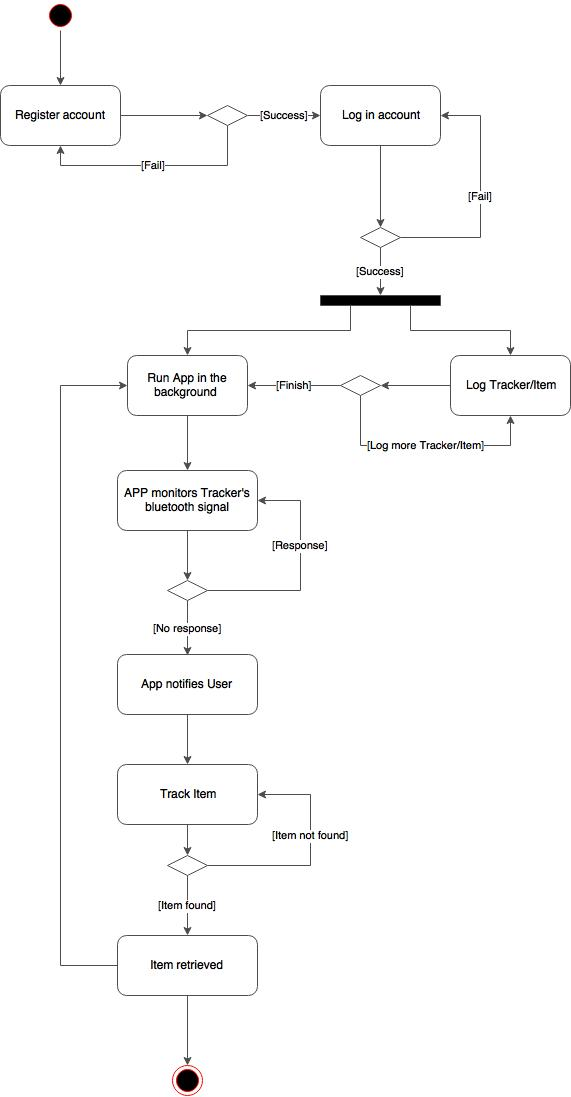
\includegraphics[width=0.7\textwidth]{assets/5-activity-diagram.jpg}
            \caption{Activity diagram}
            \label{fig:Activity diagram}
          \end{figure}
          The activity diagram shows the basic usage flow.

        \subsection{User Interface}
          We prototyped the wireframe and user interface base on the use cases with a live prototye(https://marvelapp.com/48da709) to test the usability of our design. In the proposal stage, the application provides the basic functionalities to fulfil the user needs. The user interface is listed below and sorted in usage frequency and importance.
          \begin{table}[H]
            \centering
            \resizebox{\textwidth}{!}{
              \begin{tabular}{clll}
                \hline
                ID &  Name &  Functionality &  For Use Case  \\
                \hline
                1 &  Log Item &  Log new item and Tracker to App. &  Log Tracker \\
                2 &  Item List &  Display the list &  Track Item \\
                3 &  Track Item &  Show the item's position on the map. &  Track Item \\
                4 &  Notification &  App notify User Item is lost &  Monitor Tracker \\
                5 &  Welcome &  Introduce our app to the user &  Login account. \\
                6 &  Login account&  Allow User to login account. &  Login account \\
                7 &  Register account &  User registers a new account. &  Register account \\
                \hline
              \end{tabular}
            }
            \caption{Use case index} 
          \end{table} 

          \begin{figure}[H]
            \begin{tabular}{cccc}
            \subfloat[Log Item]{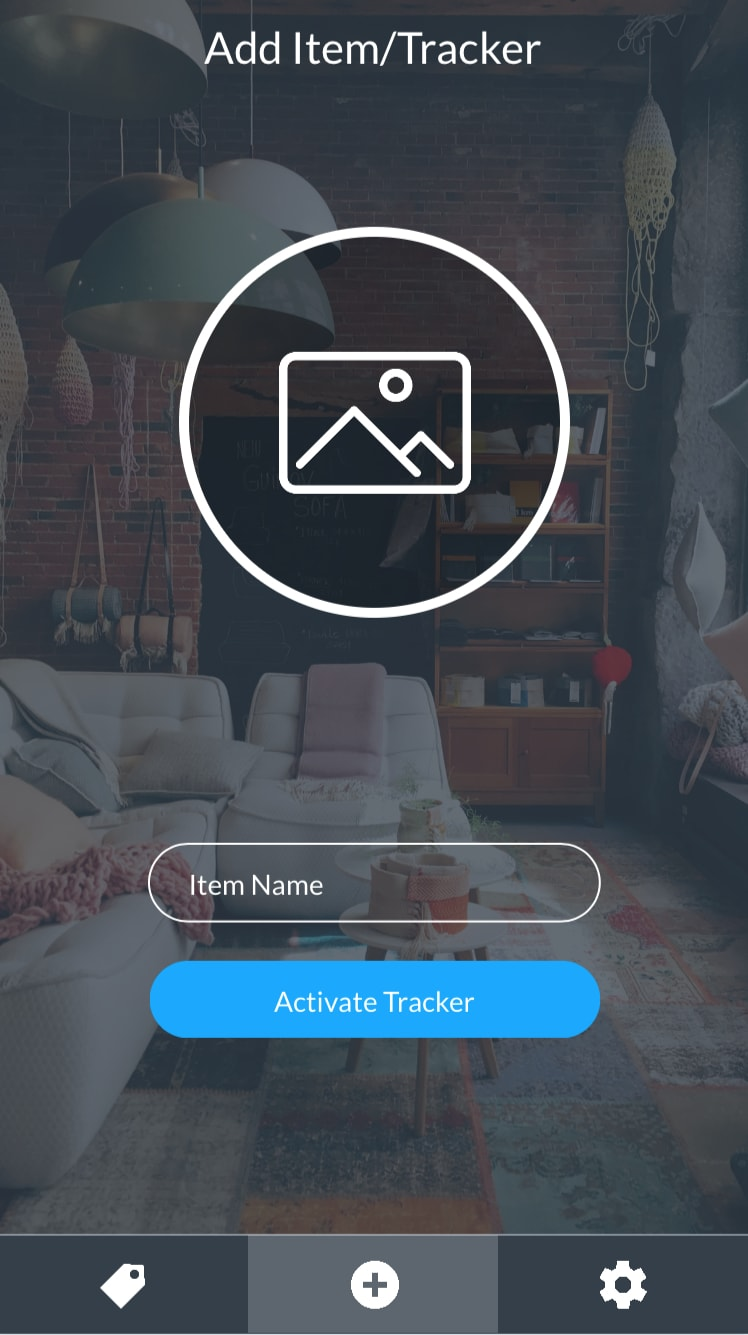
\includegraphics[width = 1.5in]{assets/5-ui-log-item.jpg}} &
            \subfloat[Item List]{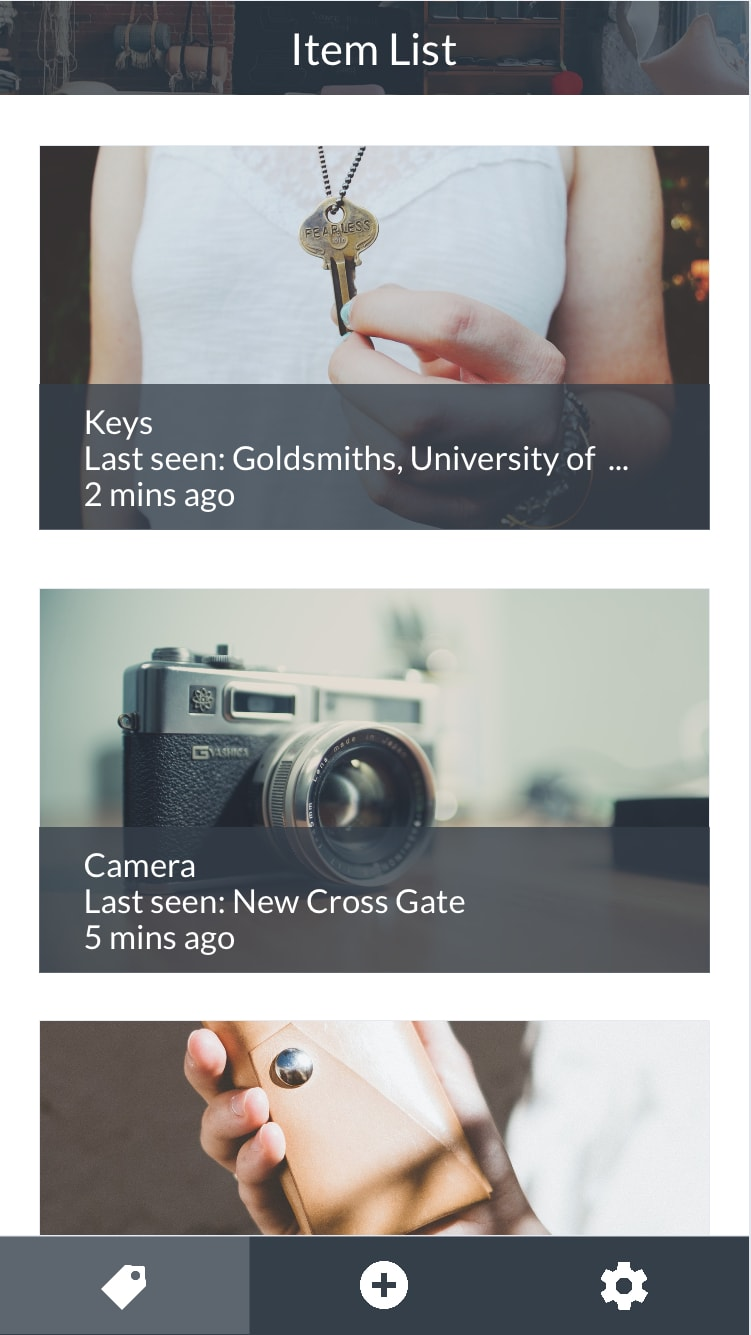
\includegraphics[width = 1.5in]{assets/5-ui-item-list.jpg}} &
            \subfloat[Track Item]{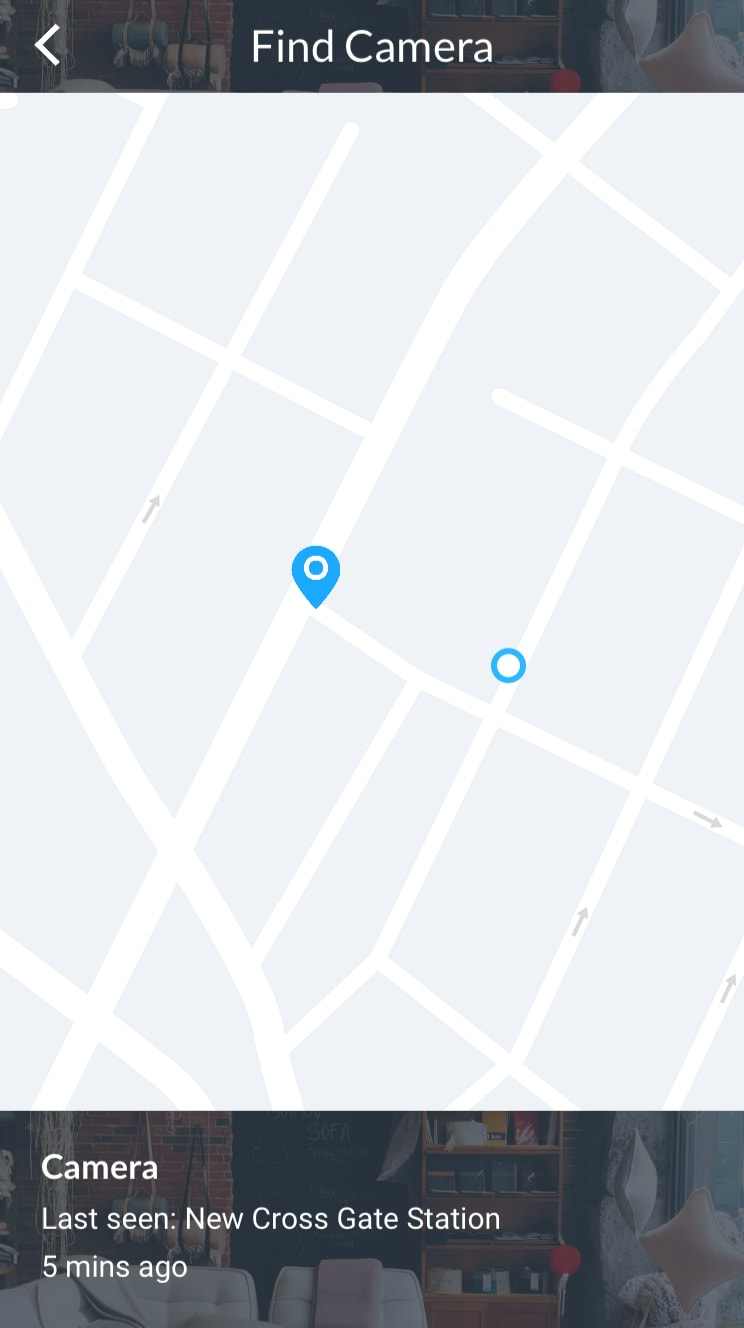
\includegraphics[width = 1.5in]{assets/5-ui-track-item.jpg}}\\
            \subfloat[Notification]{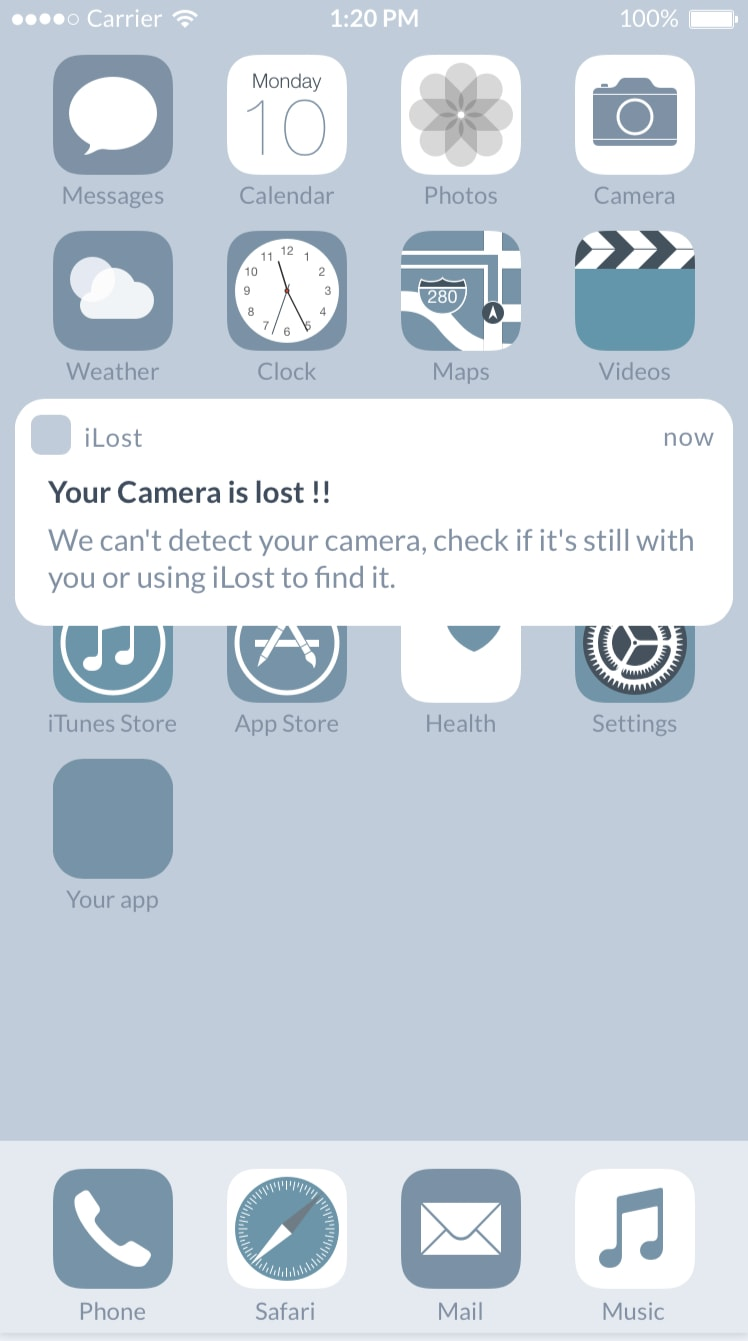
\includegraphics[width = 1.5in]{assets/5-ui-notification.jpg}} &
            \subfloat[Welcome]{
\includegraphics[width = 1.5in]{assets/5-ui-welcome.jpg}} &
            \subfloat[Login account]{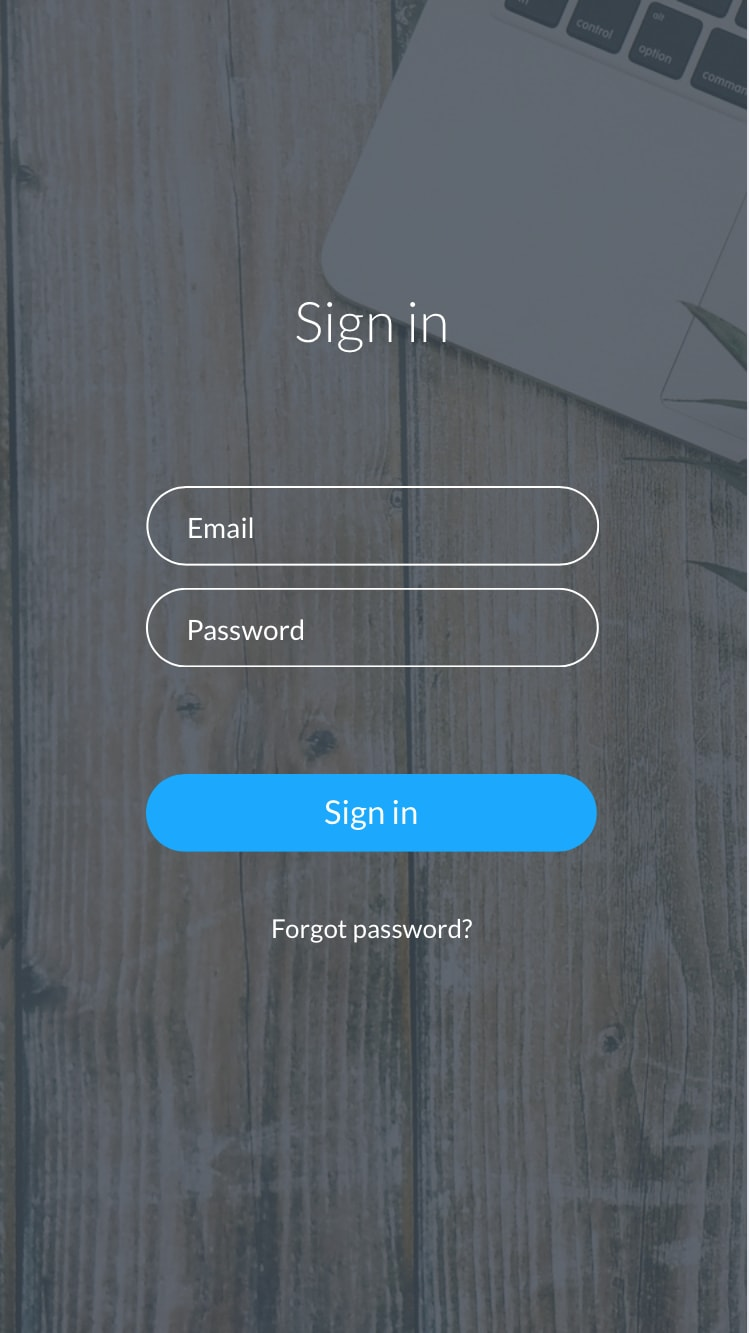
\includegraphics[width = 1.5in]{assets/5-ui-sign-in.jpg}}\\
            \subfloat[Register account]{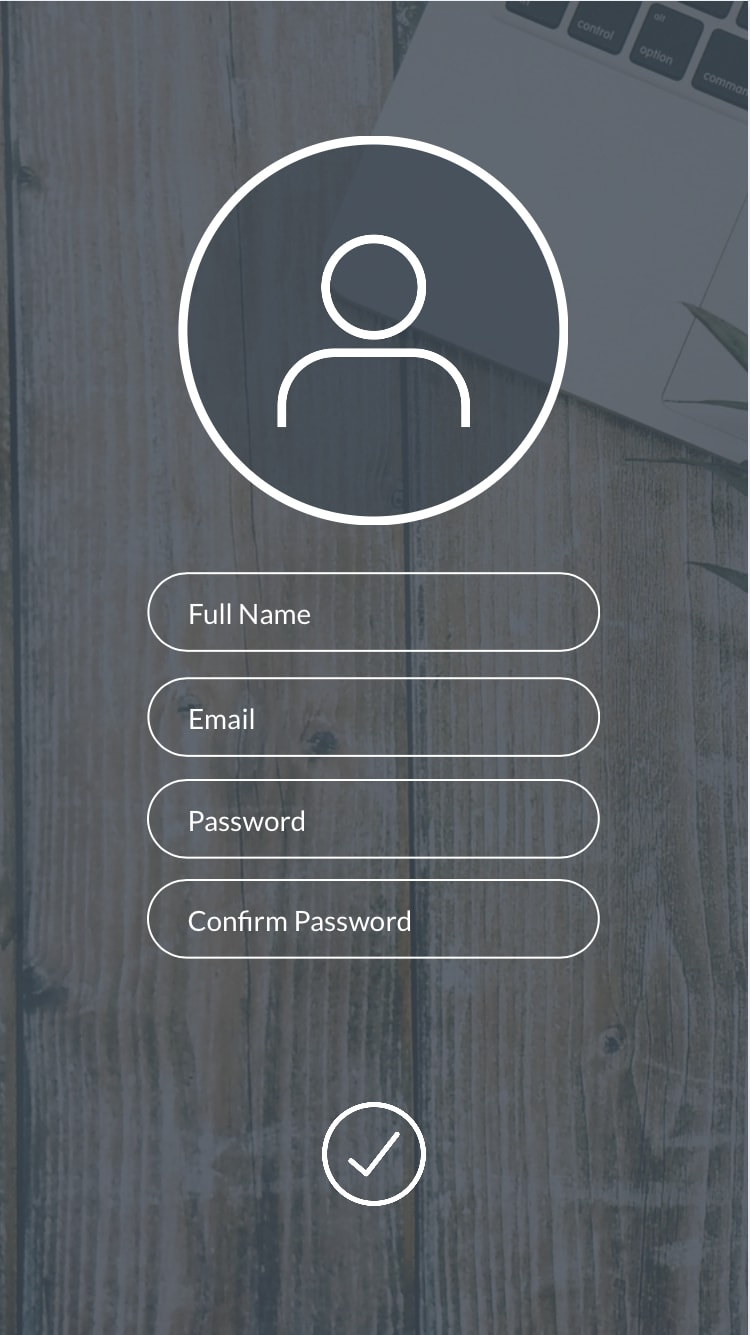
\includegraphics[width = 1.5in]{assets/5-ui-register.jpg}}\\
            \end{tabular}
            \caption{User interface design}
          \end{figure}
          
    \section{Prototyping}
      \subsection{Singular approach}
        \paragraph{}
          Initially, our orginal prototype simply consists of a Beetle BLE\cite{BlunoBeetle} (with a 3.7v battery) which pings at regular intervals to the user’s smartphone (if the ping is not detected by the smartphone after a certain time then the item is out of range)
        \paragraph{}
          We later replaced the Beetle BLE with an estimote Sticker Beacon\cite{Estimote} which has greater range and battery life as well as being relatively compact in size (also , built in 1 year battery).
        \paragraph{}
          This initial prototype did receive positive responses, however a substantial number of users stated that our product was too similar to other competitors on the market such as tile\cite{FindYourTile} etc.
        \paragraph{}
          We needed to prototype a product that was unique, Bluetooth is being overused in the market, however Bluetooth is a reliable technology at short range (0 -30 meters, users expect the tracker to last at least 6 months in the field).
        \paragraph{}
          Test prototypes were created with a GPS shield attached to an Arduino, the GPS capability was too inaccurate and power consuming. Another prototype was created using a passive and active RFID reader shield and Arduino. We discovered that either way the range was too short for the product to be feasible and too large for the user. Moreover, active RFID's are far too expensive to implement.
        \paragraph{}
          We exhausted other possibilities too. A test using acoustic location (using environmental sound to triangulate the Arduino’s location) proved that this was not feasible in the user environment (noisy – chaotic urban) and the Arduino did not have the processing capability of handling so many sound sources.
        \paragraph{}
          Moreover, we also prototyped an Arduino using wi-fi hotspots to locate itself. This proved to be unreliable as wi-fi hotspots are still not frequent enough and are not guaranteed to be operational at all times, Wi-Fi is also more power consuming than our previous prototypes. Lastly, with a cellular shield and an Arduino- we tried to manually implement cellular triangulation. This did not work for many reasons, we did not have the ability to negotiate with multiple cellular carriers and data costs would be too expensive, but we recognised that cellular was low power consuming and provided unlimited long range (cell towers cover most of the world – more than satellites or Wi-Fi hotspots).
        \paragraph{}
          After all of these singular approaches, we decided it’s best to take a Hybrid approach which allows us to exploit many of the different singular approaches we prototyped earlier.
      
      \subsection{Hybrid Approach}
        \paragraph{}
          Using Skyhook\cite{SkyhookWireless} was our first approach to prototyping using many different tracking technologies (Bluetooth, wi-fi hotspot triangulation, GPS etc..) combined. Skyhook is what the apple iPhone uses for location tracking, so it is well supported and we could use our own group member's iPhones for testing accuracy of the location tracking. The Skyhook API can be Installed on a raspberry pi or any smartphone device. It uses whatever sensors on the device to determine its location. For example, it triangulates its location from Wi-Fi hotspots, cell towers and Bluetooth signal strength.
        \paragraph{}
          The Hybrid approach does provide better location tracking, so we needed to replace Skyhook. We were inspired by the recent iTrack tracking device (the first device on the market to exclusively use cell tower triangulation). Its seemed best to combine the long range effectiveness of cellular with the excellent short range ability of Bluetooth.
        \paragraph{}
          Skyhook was replaced with Hologram Cloud\cite{Hologram}, they provide us with a small USB sized cellular modem (Hologram Nova) and a python SDK which can be installed on the raspberry pi, the modem provides cellular location data (it simplifies cell tower triangulation) which can be transmitted via 2G/3G to a Hologram cloud server. The Hologram cloud server then connects to the user’s smartphone/wearable app, sending the user the location of the tracker.
        \paragraph{}
          We tested out the python SDK and read through the documentation thoroughly.
        \paragraph{}
          Hologram Cloud does not store user data, so they charge a small amount for data usage. However, they can negotiate with carriers worldwide and provide us with automatic carrier switching.

      \subsection{Current Prototype}
        \paragraph{}
          To clarify our tracker consists of a raspberry pi, a Hologram Nova\cite{Nova} and a lithium poly battery. Bluetooth for short range and cellular triangulation for long range.
        \paragraph{}
          We developed a new protocol from this hybrid approach - In a long range situation, when the user gets closer to the tracker, less than 40 meters. The app on the user’s smartphone sends a request to Hologram cloud server, the server then sends a message to the tracker to turn on the Bluetooth module and look for the user’s smartphone/wearable thus providing a more precise location, especially in an chaotic urban environment or indoor multi-level environment. We couldn’t find any other product that provided this feature. We now need to implement and test this protocol.
    \section{Technical Architecture}          
      \paragraph{}
        The product contains three parts: a mobile application, a physical tracker and the Hologram Cloud as the server. Hologram Cloud provides various built-in functions which allow us to focus on developing the mobile application and the tracker. Due to the privacy issue, our application doesn't store any data in the cloud server or database but in the user's mobile phone only.
      \paragraph{}
        Here we provide three kinds of views in different diagrams. The process view won't be shown here because it is same as the activity diagram in the Design section.

      \subsection{Logical View}
        \begin{figure}[H]
          \centering
          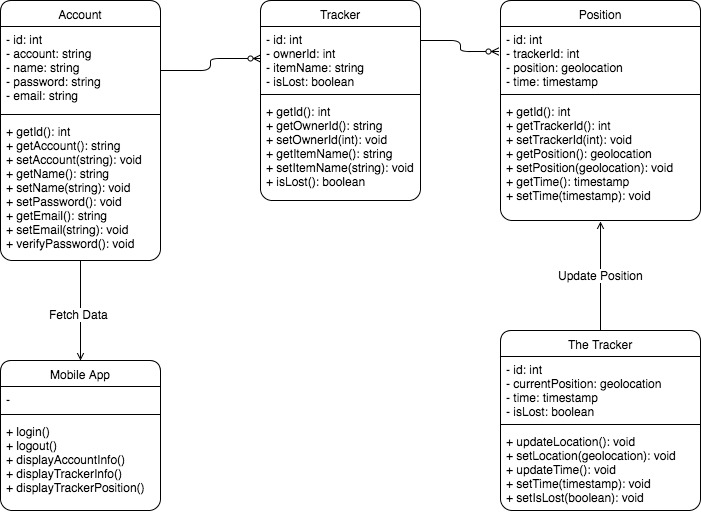
\includegraphics[width=1\textwidth]{assets/7-technical-architecture-logical.jpg}
          \caption{Logical View}
          \label{fig:Logical View}
        \end{figure}
        \paragraph{}
          The logical View diagram is based on our main architecture split into three parts: Mobile application, Hologram Cloud and Physical Tracker, and mobile application are our main focus. The architecture is based on MVC pattern, one point worth mentioning is that there are three models (Account, Tracker and Position ) while two controllers only(AccountController and TrackerController). The reason is that the Position data will be immutable and directly transferred from either Hologram Cloud or Physical Tracker, and binding the data flow with TrackerController simplify the whole routine.
        \paragraph{}
          The class of Hologram Cloud is simplified, because it comes with complex APIs and the most important function and the related functions are transferring message and updating position. The getters and setters are omitted due to the readability.
      
      \subsection{Development View}
        \begin{figure}[H]
          \centering
          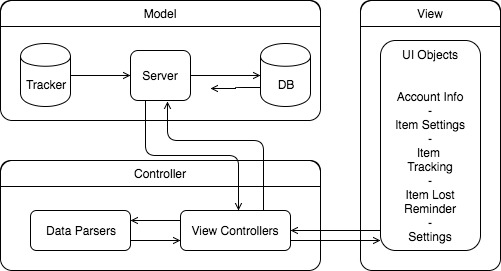
\includegraphics[width=1\textwidth]{assets/7-technical-architecture-development.jpg}
          \caption{Development View}
          \label{fig:Development View}
        \end{figure}
        \paragraph{}
         With development view, we can understand the data flow and what are the data should each component provide from a software engineer's perspective. This helps us to build a more abstract understanding of our project.

      \subsection{Physical View}
        \begin{figure}[H]
          \centering
          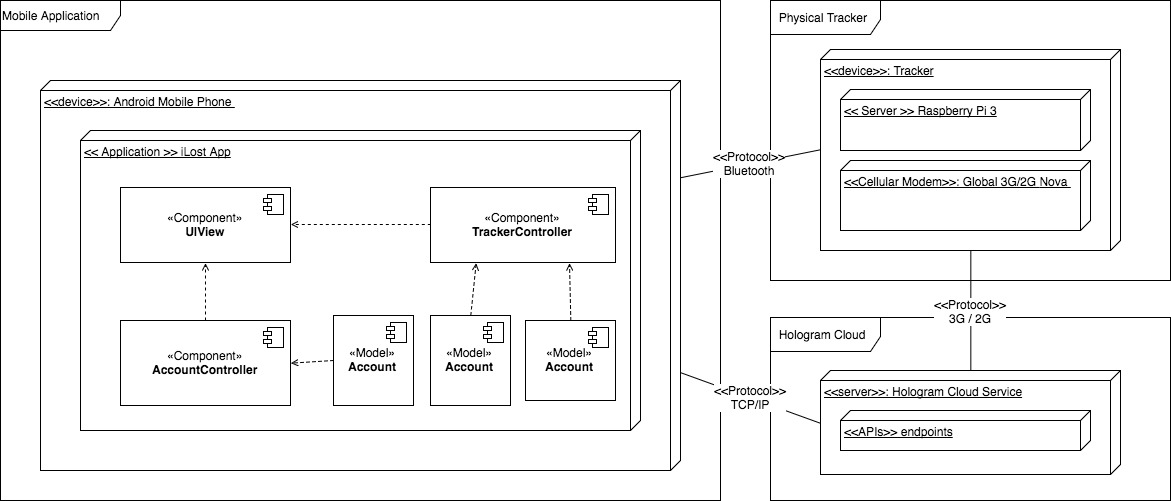
\includegraphics[width=1\textwidth]{assets/7-technical-architecture-physical.jpg}
          \caption{Physical View}
          \label{fig:Physical View}
        \end{figure}
        \paragraph{}
          The physical view is demonstrated in a deployment diagram and shows the physical structure clearly. With this diagram, we could have a more clearer overview of the whole service.
       
    \section{Evaluation Plan}
      \subsection{Hardware}
        As to the hardware, the main concern was the general size of the tracker and whether it can easily be an extension to the users’ personal items. The test cases during development are as follows;
        \begin{enumerate}
          \item Give users a mock tracker which match the dimensions of our actual tracker and then survey them as to how they feel about the size.
          \item Allow users to use the mock tracker for a week or so to determine whether they could get used to the size.
          \item Allow the user to try out different methods of attaching the tracker be it using a key ring, Velcro or adhesives and asses which they find the most convenient.
        \end{enumerate}
        The test cases post-development could be to redo the above tests and allow the users to see the effectiveness of the software and see whether the extension is worthwhile as previously they didn’t have their opinions weighed up against the actual use of the tracker.
      
      \subsection{Hardware}
      As to the software, the main concerns are the effectiveness of the Bluetooth and also the effectiveness of the cellular and whether they can withstand extreme measures. The test cases during development are as follows;
      \begin{enumerate}
        \item The notification a user receives in multiple scenarios such as a loud club, a library and at home and see whether the notification is adequate to grab the users’ attention.
        \item The accuracy of the distance the Bluetooth trackers tells the user by thoroughly testing different locations.
        \item The ability of the hologram to triangulate the location in areas with poor cellular signal.
        \item Its ability to give a location within a radius of 10m.
      \end{enumerate}
      The test cases post development will have to be more thorough so we can identify bugs and typical usage problems early in the beta stage before we push the first version and thus assure quality of the product is maintained and optimal.
          
    \section{Project Management}
      \subsection{Project Cycle}
      \begin{figure}[H]
        \centering
        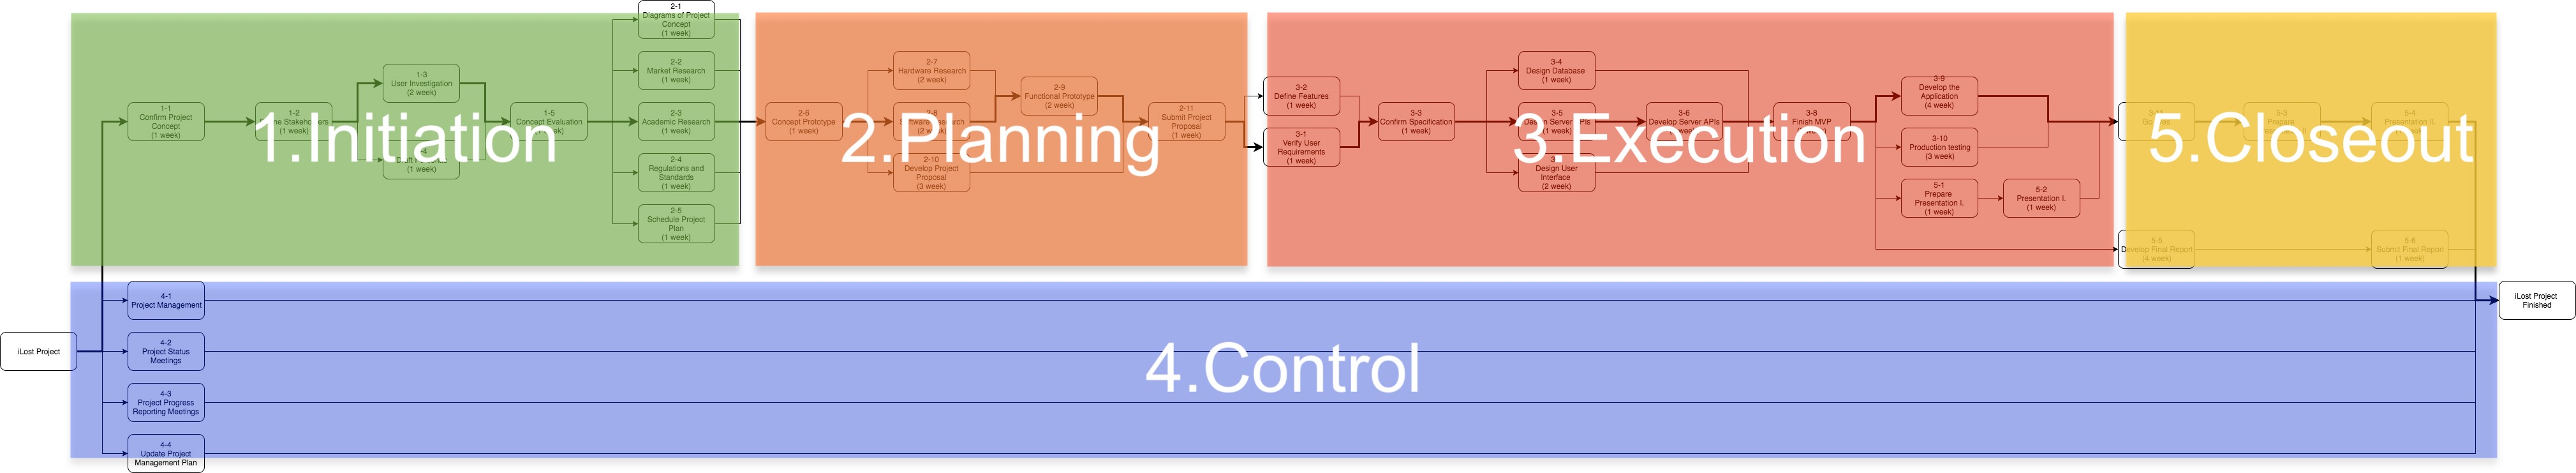
\includegraphics[width=1\textwidth]{assets/9-project-diagram-all.jpg}
        \caption{Project Diagram All}
        \label{fig:Project Diagram All}
      \end{figure}
      \paragraph{}
        Our project cycle contains five process groups\cite{pmp} and three milestones at the end of some of the developing process. "Initiation" and "planning" two stages are before the proposal submission, "execution" is for developing the actual product, "control" is for project management and "closeout" is the for the final presentation and report.
      
        \begin{table}[H]
          \centering
          \resizebox{\textwidth}{!}{
            \begin{tabular}{cl}
              \hline
              Stage &  Description \\
              \hline
              Initiation & Confirming the project concept, personas and user needs. \\
              Planning & Researching technology and developing the proposal. \\
              Execution & Developing the minimum viable product and final production. \\
              Control & Project management and the weekly meetings. \\
              Closeout & Developing presentation and final report. \\
              \hline
            \end{tabular}
          }
          \caption{Stage Descriptions} 
        \end{table} 

        \begin{figure}[H]
          \centering
          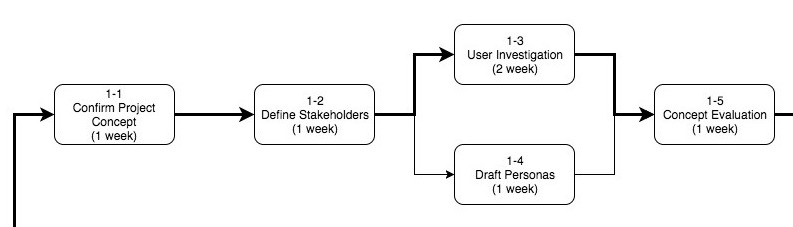
\includegraphics[width=1\textwidth]{assets/9-project-diagram-1.jpg}
          \caption{Project Diagram Initiation}
          \label{fig:Project Diagram Initiation}
        \end{figure}

        \begin{figure}[H]
          \centering
          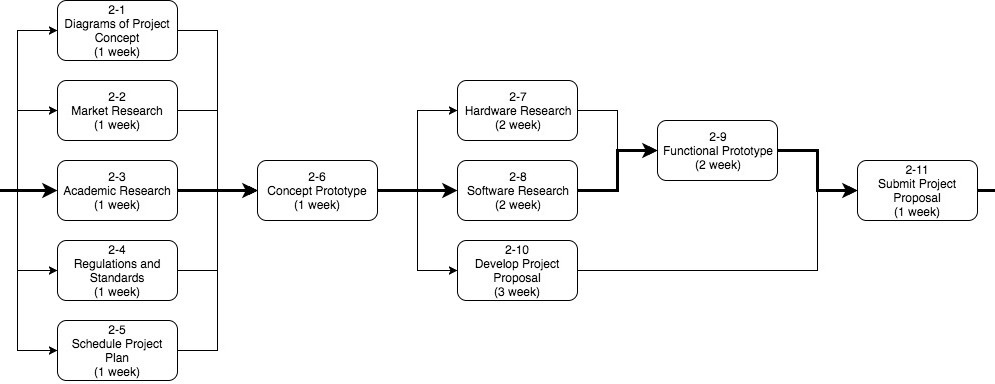
\includegraphics[width=1\textwidth]{assets/9-project-diagram-2.jpg}
          \caption{Project Diagram Planning}
          \label{fig:Project Diagram Planning}
        \end{figure}

        \begin{figure}[H]
          \centering
          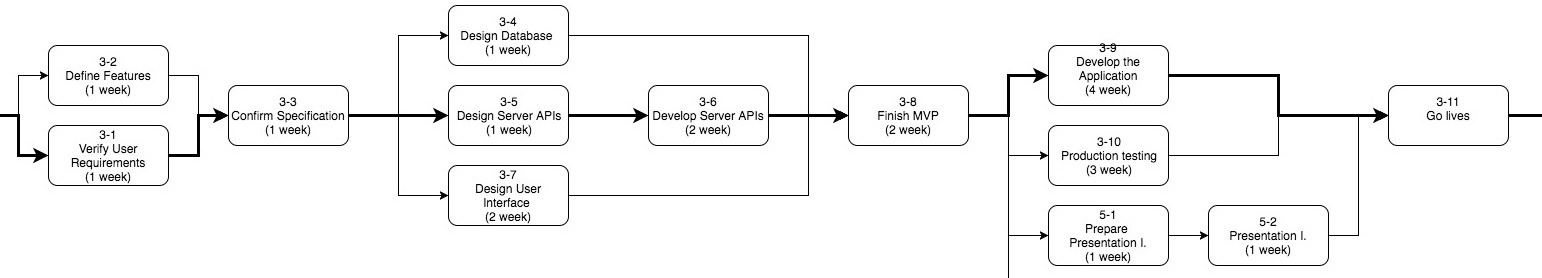
\includegraphics[width=1\textwidth]{assets/9-project-diagram-3.jpg}
          \caption{Project Diagram Execution}
          \label{fig:Project Diagram Execution}
        \end{figure}

        \begin{figure}[H]
          \centering
          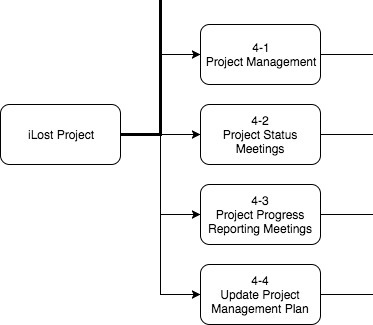
\includegraphics[width=.5\textwidth]{assets/9-project-diagram-4.jpg}
          \caption{Project Diagram Control}
          \label{fig:Project Diagram Control}
        \end{figure}

        \begin{figure}[H]
          \centering
          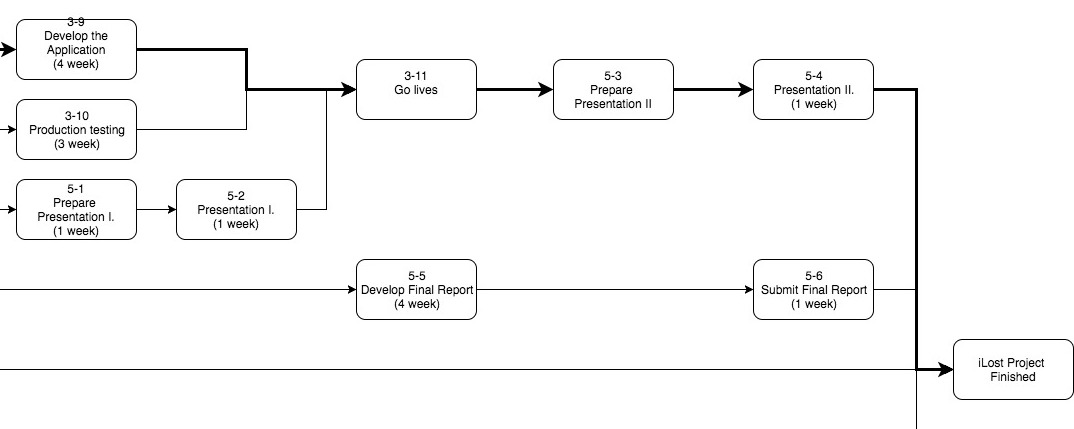
\includegraphics[width=1\textwidth]{assets/9-project-diagram-5.jpg}
          \caption{Project Diagram Closeout}
          \label{fig:Project Diagram Closeout}
        \end{figure}

        Each stage contains multiple tasks which we used to create Gantt chart and record our progress tracking form. More details about the tasks is in Appendix \ref{appendix:project-tasks-list}. The project also contains three main milestones end at different stage.  

        \begin{table}[H]
          \centering{
            \begin{tabular}{ll}
              \hline
              Milestone Name & Stage \\
              \hline
              Project Proposal & End of Planning \\
              Project Application &  End of Execution \\
              Project Final Proposal & End of Closeout \\
              \hline
            \end{tabular}
          }
          \caption{Milestones} 
        \end{table} 

      \subsection{Gantt Chart}
        \begin{figure}[H]
          \centering
          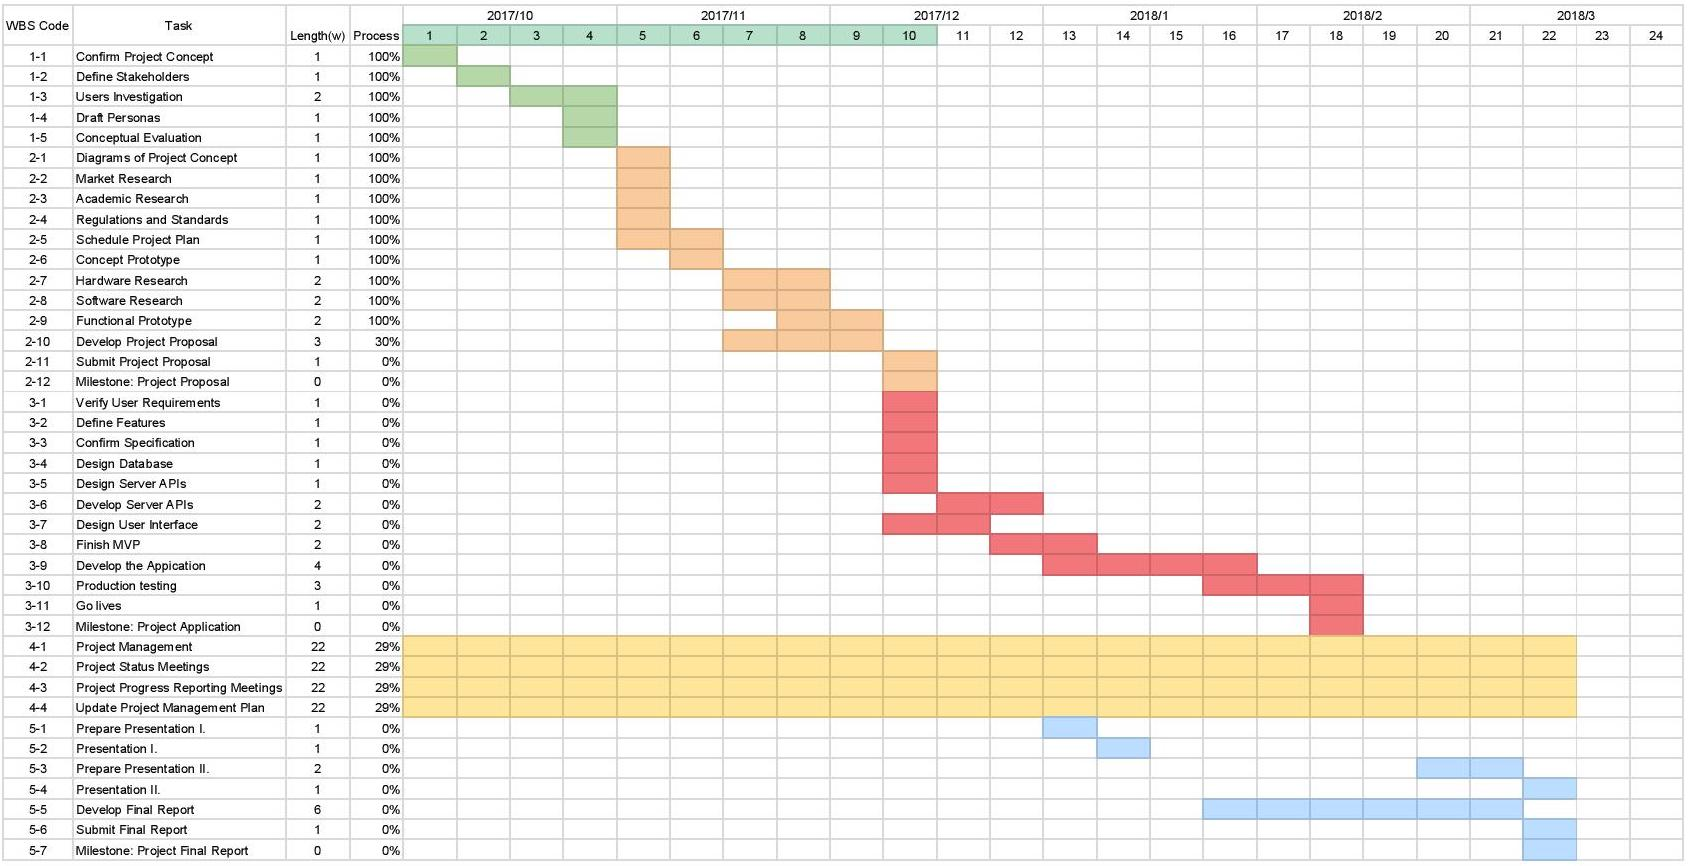
\includegraphics[width=1\textwidth]{assets/9-gantt-chart.jpg}
          \caption{Gantt Chart}
          \label{fig:Gantt Chart}
        \end{figure}
        \paragraph{}
          The Gantt chart was created based on the task list, using a week as a minimum developing unit to measure and schedule the developing process is more feasible than using day and more preciser than using a month.
        \paragraph{}
          Our weekly routine and meeting notes are in the Appendix \ref{appendix:weekly-routine} and \ref{appendix:meeting-notes}
      
      \subsection{Project Management Tools}
        \paragraph{}
          Slack, Trello, Google Sheets and Github are our main project management tools to fulfil various developing needs. After using Github to record our weekly reports and cooperate on proposal, it's not necessary to use Trello. Github has the features we need from Trello, so we are considering to replace Trello with it completely in the next stage. 
        \paragraph{}
          Full progress tracking form can found in Appendix \ref{appendix:progess-tracking-form} and \ref{appendix:progess-tracking-charts}. More details about how we utilise all the tools and workflow are in Appendix \ref{appendix:project-management-tools-details}, \ref{appendix:github-directories} and \ref{appendix: github-workflow}.
      \subsection{Roles}
        \paragraph{}
          There are only two types of roles: project manager and project team member. Still it's inevitable for the project manager to do the same duties as the project member.
        \paragraph{}
          More details about the roles are in Appendix \ref{appendix: roles}.

    \section{Conclusion}
      \paragraph{}
      As established by our survey and research by Mozy, we believe the loss of personal belongings in various places is a common, daily life problem for majority of people.
      \paragraph{}
      Our solution to this problem is a tracker that works at short and long range, which the user can interact through a mobile application to keep track of an item. Other products on the market, don't provide a short and long range tracker, or a tracker that adapts to the user. 
      \paragraph{}
      From our survey, we predict a majority of target users will be individuals who are always on the move and active, such as students, office workers who many times need to travel abroad. 
      \paragraph{}
      Prototyping with different technologies we concluded that only one type of technology wouldn’t meet our concept prototype; therefore, we sought a hybrid solution. A combination of Bluetooth at short range and cellular at long range.
      \paragraph{}
      We recognise our product may raise privacy concerns. To address this a ‘terms of use’ script will be ensuring consumers that their data and location will be used for the sole purpose of retrieving items or help them prevent losing them. In order that our product satisfies all our use cases, we will have to experiment and test the UI of our product as well as the underlying physical architecture.
      \paragraph{}
      As of now, the lack of resources and expertise are limiting us to build a more portable physical device. We hope to deliver an upgraded version of the device in future after conducting further research on our concept, following the development of the working prototype.

    \begin{thebibliography}{20}
      \bibitem{LostAndFound} Lost \& Found – Data Loss Research – Mozy.uk. [Online]. Available: https://mozy.co.uk/about/news/reports/lost-and-found. [Accessed: 01-Dec-2017].      
      \bibitem{BlunoBeetle} Bluno Beetle. [Online]. Available: https://www.dfrobot.com/wiki/\\index.php/Bluno\_Beetle\_SKU:DFR0339. [Accessed: 15-Nov-2017].
      \bibitem{Estimote} “What are Estimote Stickers?,” Estimote Community Portal. [Online]. Available: https://community.estimote.com/hc/en-us/articles/203323543-What-are-Estimote-Stickers-. [Accessed: 29-Nov-2017].
      \bibitem{FindYourTile} “Find Your Tile,” Waterproof Tile Sport Bluetooth Tracker Helps You Find Your Things | Tile. [Online]. Available: https://www.thetileapp.com/en-gb/products/sport. [Accessed: 30-Oct-2017].
      \bibitem{SkyhookWireless} “Skyhook Wireless | Location data provider,” Skyhook Wireless | Location data provider. [Online]. Available: http://www.skyhookwireless.com/. [Accessed: 27-Oct-2017].
      \bibitem{Hologram} “Cloud services,” Hologram. [Online]. Available: https://hologram.io/cloud/. [Accessed: 01-Dec-2017].
      \bibitem{Nova} “IoT \& M2M Cellular Modem for Raspberry Pi – 2G/3G/4G LTE Cat-M1,” Hologram. [Online]. Available: https://hologram.io/nova/. [Accessed: 02-Dec-2017].
      \bibitem{pmp} Kanata and Ont, Project management professional (PMP), 1st ed. Beacon Associates Publications, 2004.
      
    \end{thebibliography}
    
    
    \begin{appendices}      
      \section{Use Case Flow}
      \label{appendix:use-case-flow}
        \subsection{Log trackers}
          \paragraph{Basic Flow}
          \begin{enumerate}
            \item User attachs Tracker to a personal item.
            \item App links to Tracker with bluetooth.
            \item App activates Tracker.
            \item User logs details of the item and Tracker in App.
            \item App validates and saves the inputs.
          \end{enumerate}
        
          \paragraph{Alternative Flows}
          \begin{itemize}
            \item Multiple Trackers: After Step 4, repeat step 1 to 4 for additional Trackers and items.
          \end{itemize}
        
        \subsection{Monitor Tracker}
          \paragraph{Basic Flow}
            \begin{enumerate}
              \item App listens for signal at regular intervals.
              \item App saves the history of the position of Tracker at regular intervals.
            \end{enumerate}
          \paragraph{Alternative Flows}
          \begin{itemize}
            \item Tracker is with user: If Tracker is within certain distance from User, App listens for bluetooth singal.
            \item Tracker is lost: Tracker is not within certain distance from User.
            \begin{enumerate}
              \item App activates Tracker's cellular mode via bluetooth.
              \item App sends a notification to mobile OS to nofity User.
              \item App listens for the geolocation data of Tracker sent from Server.
            \end{enumerate}    
            \item Tracker is nearby but not with User after being lost: Tracker is within bluetooth dectable distance after being far away from User.
            \begin{enumerate}
              \item App activates Tracker's bluetooth mode via Server.
              \item App listens for the geolocation data of Tracker sent from Server and bluetooth singal at the same time.
            \end{enumerate}    
            \item Tracker is with User after being lost: App deactivates Tracker's cullular mode via bluetooth, then Resume at Base Flow step 1.
          \end{itemize}
          
        \subsection{Track Item}
          \paragraph{Basic Flow}
            \begin{enumerate}
              \item User selects desired tracking item in App.
              \item App displays the position data of Tracker.
            \end{enumerate}
      
        \subsection{Send position data}
        \paragraph{Basic Flow}
          Tracker sends position data to App.
        \paragraph{Alternative Flows}
          \begin{itemize}
            \item Activates Cellular mode: Tracker's bluetooth signal is not reaching App after a period of time, then App send message via Server to activates cellular mode.
            \item Bluetooth mode is activated: Tracker sends position data via bluetooth to App.
            \item Cellular mode is activated: 
            \begin{enumerate}
              \item Tracker sends position data via cellular to Server.
              \item Server transfer the position data to App.
            \end{enumerate}    
          \end{itemize}
      
      
      \subsection{Register account}
      \paragraph{Basic Flow}
        \begin{enumerate}
          \item User input account details.
          \item App validates the inputs.
          \item App creates a new account.
        \end{enumerate}
      \paragraph{Alternative Flows}
        \begin{itemize}
          \item Inputs are validated failed: After step 2, resume at step 1 if the inputs are not validated.
        \end{itemize}
      
      \subsection{Login account}
      \paragraph{Basic Flow}
        \begin{enumerate}
          \item User input account details.
          \item App validates the inputs.
          \item App allows User to login.
        \end{enumerate}
      \paragraph{Alternative Flows}
        \begin{itemize}
          \item Inputs are validated failed: After step 2, resume at step 1 if the inputs are not validated.
        \end{itemize}
    
    \section{Hardware Research}
     \label{appendix:hardware-research}
    \subsection{Bluetooth Component module}
      \paragraph{}
      Bluetooth has established itself as the wireless communication standard of choice to connect wearable devices to smartphones, tablets or PCs,
      \paragraph{}
      The SESUB-PAN-D14580 module, which is based on TDK's SESUB (semiconductor embedded in substrate) integration technology, features an embedded DA14580 Bluetooth 4.1 chip from Dialog Semiconductor. All terminals of the discrete chip are available, allowing full use of chip functions
      \paragraph{}
      The module features an integrated DC-DC converter. With a voltage supply of 3.0 V, its current consumption is only 5.0 mA when transmitting, 5.4 mA when receiving and 0.8 µA in standby mode.
      \paragraph{}
      The ultra-compact dimensionsTDK SESUB-PAN-D14580 module are just 3.5 mm x 3.5 mm x 1.0 mm.
      \paragraph{Main features and benefits}  
      \begin{enumerate}
        \item Ultra compact module dimensions of 3.5 mm x 3.5 mm x 1.0 mm (typical) drastically reduces the mounting footprint to only about 12 mm2
        \item Easy implementation of Bluetooth connectivity
        \item Integrated DC-DC converter
      \end{enumerate}
    
    \subsection{Active RFID tag}
      \paragraph{}
        Active RFID systems have three essential parts – a reader or interrogator, antenna, and a tag. Active RFID tags possess their own power source – an internal battery that enables them to have extremely long read ranges as well as large memory banks.
      \paragraph{}
        Typically, active RFID tags are powered by a battery that will last between 3 – 5 years Essentially, two different types of active RFID tags are available – transponders and beacons.
      \paragraph{Transponders} 
        In a system that uses an active transponder tag, the reader (like passive systems) will send a signal first, and then the active transponder will send a signal back with the relevant information. Transponder tags are very efficient because they conserve battery life when the tag is out of range of the reader. Active RFID transponders are commonly used in secure access control and in toll booth payment systems.
      \paragraph{Beacons} 
        In a system that uses an active beacon tag, the tag will not wait to hear the reader’s signal. Instead, true to its name, the tag will ‘beacon’, or send out its specific information every 3 – 5 seconds. Beacon tags are very common in the oil and gas industry, as well as mining and cargo tracking applications. Active tag’s beacons can be read hundreds of meters away, but, in order to conserve battery life, they may be set to a lower transmit power in order to reach around 100 meters read range.
      \paragraph{Estimote} 
        An Estimote Beacon is a small, wireless device, when placed in a physical space, it broadcasts tiny radio signals to smart devices.
      \paragraph{} 
        Estimote Beacon is like a small computer. Its 32-bit ARM® Cortex M0 CPU is accompanied by accelerometer, temperature sensor, and what is most important—2.4 GHz radio using Bluetooth 4.0 Smart, also known as BLE or Bluetooth low energy. This is able to provide mobile devices in range with information about their location and state.
      \paragraph{} 
        Estimote is an iBeacon-compatible hardware transmitters, using the idea of smart objects that work as transmitter to broadcast digital data using Bluetooth Smart protocols:
      \begin{enumerate}
        \item Eddystone UID
        \item Generic Advertiser
        \item Nearable
        \item Estimote Monitoring
        \item iBeacon
      \end{enumerate}
      \paragraph{}
        iBeacon is a Bluetooth advertising protocol designed by Apple, with native support in iOS, a specification that tells what data, and in what format, a Bluetooth beacon needs to advertise. Estimote Monitoring is the default protocol in both Location and Proximity Beacons and it was built as a mix of Estimote Location and iBeacon, taking the best features of both protocols. It offers various improvements in accuracy and beacon detection and is currently the most reliable protocol
  
      \paragraph{Pros}
        \begin{enumerate}
          \item Extremely Long Read Range
          \item Increased tag abilities with partnered technologies (GPS, sensors, etc.)
          \item Extremely Rugged tag options
        \end{enumerate}
  
    \subsection{IBeacon Technology (Bluetooth Low Energy Tags)}
      \subsubsection{Accessibility}
        \paragraph{}    
          With smartphones primarily acting as receivers, beacons form a highly accessible indoor location technology.
          \paragraph{Pros}    
          The capability of beacons to allow smartphones to primarily act as the receivers, makes it a highly accessible location technology
          \paragraph{Cons}    
          Beacons once installed need to be checked regularly for battery levels, making this less practical.
          \paragraph{Range}
          Beacons typically have a wireless range of 1m to 70m
          \paragraph{Accuracy}
          Beacons being radio transmitters are not very accurate as they stand the chance of interference, as radio signals can be absorbed by different media, such as water, air, human bodies or even metallic surfaces Cons: Beacons being radio transmitters are prone to suffer from interference
          \paragraph{Security}
            \subparagraph{Pros}
              No intrinsic security risks. Since beacons are primarily proximity detection devices that broadcast outbound signals, there is no inherent security risk in the transmission.
            \subparagraph{Cons}
              The Signals sent out by beacons can be intercepted and used by hackers. Most manufacturers have built in countermeasures that attempt to counter this.
          \paragraph{Cost}
            While beacons by themselves are relatively cheap (a typical beacon would cost you anywhere between £5 to £50), the number of beacons required depends on the size of the space and range needed. The cost of beacon system depends on several other factors such as app and integration cost, licensing and data service cost. 
    
    \subsection{Bluetooth 5}
      Although We don’t believe Bluetooth 5 is currently established. The Bluetooth 5 update will bring:
      \begin{itemize}
      \item 4x the range
      \item 2x the speed
      \item 800\% more broadcast messaging capacity
      \end{itemize}
    
    \subsection{Cellular}
      \paragraph{}
      A great advantage of cellular is its long range, it comes second to GPS for range. Our product will be used in an unpredictable urban environment. Cell phone towers are everywhere in an urban and even sub-urban environment. Cellular requires less energy than Wi-Fi and does not require a WPA/WEP key (or any other login system) to fully exploit.
      \paragraph{}
      However, a tracker using Cellular will require a bigger antenna than what a wi-fi tracker currently uses. During research we discovered whenever a tracking device was using Cellular networks it was in fact using 2G (3G, 4G etc.) to connect to the internet (this is expensive and defeats the purpose of using cellular in this context). What we really want is a Cellular tracker to use triangulation from different cell phone towers to pinpoint its own location.
      \paragraph{}
      Government agencies such as intelligence services and emergency services use Cellular triangulation, through our research we found that it would not be possible to implement cellular triangulation in the same way Government/emergency agencies do, we lack expertise knowledge, resources and connections.
      \paragraph{}
      But, we have found a “middle-man” who can, so to speak. SkyHook, the same location provider Apple uses, also provide cell phone triangulation using a map of cell phone towers, they also use the same technique with wi-fi hotspots.
    
    \subsection{Acoustic Location}
      \paragraph{}
        Sound waves travel at an average 343 m/s. By detecting the time taken for the phone (which is what the user interacts with) to detect a sound (which is an inaudible frequency emitted at regular time intervals by the tracker) we can work out the average location of the tracker: distance (m) = speed(m/s) * time (s).
      \paragraph{}
        A unique approach, its currently only extensively used by the military and emergency rescue teams. The problem is that the product environment (chaotic Urban) has to much sound interference, this will severely limit the smartphones microphone ability to distinguish the inaudible frequency emitted by the tracker. We also need more than one “listening” device to make triangulation possible.
      \paragraph{}
        In environments were acoustic location is possible, high grade/ large microphones are used and they are normally used in an open or quieter environment than a chaotic urban environment which this product is designed for.

    \subsection{Hybrid Server Side – SkyHook implementation}
      \paragraph{}
        Whatever device (android, iOS, wearable, any modern operating system) SkyHook can use the device Wi-Fi/cellular/GPS capability and to find the precise location of the device. It does this by mapping wi-fi hotspots, cell phone towers and/or GPS which the device comes across. By using this map, SkyHook can triangulate the location of the device, thus providing a precise location. The iPhone location capability is actually provided by SkyHook.
      \paragraph{}
        The device, in this case our product, the SkyHook APK maps nearby WI-FI hotspots and cell phone towers and use this data to triangulate were the location of the device is. It can also add GPS data (but our product may not have GPS capability) SkyHook is only part of the product, a tracker still needs to interact with SkyHook’s servers.
      \paragraph{}
        SkyHook data is stored in the United States raising privacy concerns, however SkyHook has “Skyhook has certified to the EU-U.S. Privacy Shield Framework for the transfer of Personal Information from the EEA to the United States” so we can still deploy using SkyHook
    
    \subsection{RFID (Radio Frequency Identification) systems}
      \paragraph{}
        Passive RFID systems use tags with no internal power source and instead are powered by the electromagnetic energy transmitted from an RFID reader.
      \paragraph{}
        Made up of two main components – the tag’s antenna and the microchip or integrated circuit.
      \paragraph{}
        There are three main frequencies within which passive RFID tags operate: 
        \begin{itemize}
          \item 125 -– 134 KHz -– Low Frequency (LF) range : 1 -– 10 centimeters. 
          \item 865 –-– 960 MHz -– Ultra High Frequency (UHF) range: 5 -– 6 meters
          \item 13.56 MHz -– High Frequency (HF)
          \item Near-Field Communication (NFC)range: 1 centimeter up to 1 meter. 
        \end{itemize}
      \paragraph{Pros}
        Smaller tags Much cheaper tags (starting from £1 - £20+) Thinner/more flexible tags Higher range of tag options Tags can last a lifetime without a battery (depending on the wear and tear)
      \paragraph{Cons}
        The tag can be read only at short distances. Passive tags have difficulty sending data through liquids or metal. The orientation of a passive RFID tag must be just right or the reader won't locate it.
      \paragraph{}
        Active RFID systems use battery-powered RFID tags that continuously broadcast their own signal (like a cell phone). Made up of three essential parts – a reader (or interrogator), antenna, and a tag.There are two main frequencies used by active systems – 433 MHz and 915 MHz
      \paragraph{Pros}
        Extremely Long Read Range Increased tag abilities with partnered technologies (GPS, sensors, etc.) Extremely Rugged tag options It can have more memory to, store more data. Cons of Passive RFID: Sensitive to harsh environment Costs more (starting from 15/20£ a piece) Larger size and weight.
      \paragraph{Conclusions}
        Either RFID system has advantages and disadvantages of their own, depending on needs.
      \paragraph{}
        Speaking for our purpose an active ultra-wideband (UWB) RFID system, would be able to determine a tagged objects location within few inches. But UWB tags are really expensive.
      \paragraph{}
        A passive UHF RFID system can provide about 5 - 10 metres of read range (distance from which a reader can communicate with tag). These can tell the tag is within a read field, but not specifically where within the field.
      \paragraph{}
        Passive RFID system uses something called Received Signal Strength Indicator (RSSI) to determine how close the tagged object is to the RFID interrogator. RSSI can’t tell if tag is, for example 20 cm away, but it can tell if tagged object is getting closer or further away.
    
    \subsection{Arduino GPS}
    \paragraph{}
      There are many Arduino GPS hardwares out in the market that are buyable. The prices of the GPS Arduino hardwares depends on usually the spec that they have. The hardware will be incorporated with the other features that our initial product will carry. Looking into the market, not one GPS Arduino hardware is perfect, however some excel above all the others. Popular builds so far for the Arduino GPS have been the Copernicus, LS23060, D2523, SUP500F, MN5010 (uMini) and EM-406A. All if not most GPS, are connected via satellites, to get a broad understanding of how each of these look and what they display on a map it is best recommend to configure Google 2D Maps along with a side to side 2D analysis.
    \paragraph{}
      The one flaw that these GPS Arduino hardwares have is that inside a structure the signal might not give off an accurate pinpoint location.
      \begin{figure}[H]
        \centering
        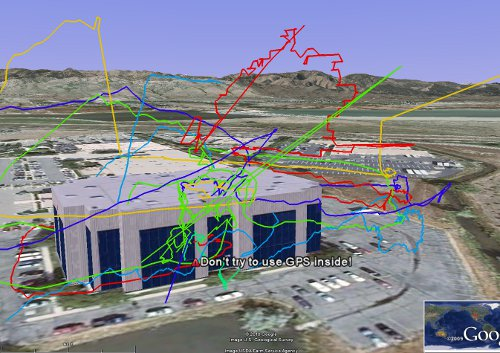
\includegraphics[width=1\textwidth]{assets/12-6-1-gpsinside.jpg}
        \caption{GPS Tracking}
        \label{fig:GPS Tracking}
      \end{figure}
    \paragraph{}
      This image \ref{fig:GPS Tracking} shows why at first call someone should not use a GPS Arduino hardware inside as signals are distraught. Also why someone should not try to access a area inside a structure even if they are outside. The different colours are the different modules that are mentioned above and how they react to finding a location from inside a structure or a location in the structure. However, there is a likely solution for this. You can attach other elements to the Arduino GPS hardware, a user will have to program a solution on how to make the signals content and not overly responsive. This is only for being able to use the Arduino GPS hardware from inside a structure. Coding something to pinpoint a location within a structure is far more complicated.

      \begin{table}[H]
        \centering
          \begin{tabularx}{\textwidth}{ccXX}
            \hline
            Modules  & Price & Pros & Cons   \\
            \hline
            Copernicus  & £56 & Basic Understanding of code, at least be able to code serial or TTL. One of the most accurate and reliable modules. It evaluates data in all conditions.   & A good understanding of electrical prototyping as user will need to know how much power is required, what each pin does, how to hook up the hardware, etc.   \\\hline
            LS23060  & £45 & This requires a good understanding of code, at least be able to code serial or TTL. Tracks longitude and latitude in all conditions. This module also has a good evaluation in all conditions.   & A well understanding of electrical prototyping due to users needing to know how much power is r\\\hline
            D2523  & £60  & This requires a well round understanding of code, at least be able to code serial or TTL. Good at places where it is hard to get a signal due to certain conditions such as a high source of dielectric materials. - Excellent latitude and longitude when the sky is clear. Similarly with data ev\\\hline
            SUP500F  & £35 & The hardware (module) is very small. - Due to its size, it also does not take too much power. &  Not having a lot of power can also be an disadvantage. \\\hline
            MN5010 (uMini) & £55 & This hardware is also very small, therefore it does not take up a lot of space. Allows both hot start and cold start. & Connection is not as accurate as it uses chip antenna. \\\hline
            EM-406A  & £48 & Allows for all 3 start up times.  & - Requires and will take up a lot of power. Likely to be interference due to it connecting via chip antenna.  \\
            \hline
          \end{tabularx}
        \caption{Pros \& Cons of Modules} 
      \end{table} 

      \section{Project Tasks List}
        \label{appendix:project-tasks-list}
        \begin{longtable}{p{2cm}p{1cm}p{3cm}cp{6cm}}
          \hline
          Major Task & WBS Code & Task & Length(w) & Definition\\
          \hline
          Initiation & 1-1 & Confirm Project Concept & 1 & Team brainstorms and confirms the concept of the project\\\hline
          Initiation & 1-2 & Define Stakeholders & 1 & Consider the stakeholders that might be relevant.\\\hline
          Initiation & 1-3 & Users Investigation & 2 & Investivate the prospect users' need and opinions.\\\hline
          Initiation & 1-4 & Draft Personas & 1 & Draft personas that might represent a typical user for the ideas.\\\hline
          Initiation & 1-5 & Conceptual Evaluation & 1 & Decide wheather to continue the project.\\\hline
          Planning & 2-1 & Diagrams of Project Concept & 1 & Produce use case diagrams, use scenarios, sequence diagrams and activity diagrams.\\\hline
          Planning & 2-2 & Market Research & 1 & Search for competing products directly and from reviews, trade sites, press reviews and customer reviews.\\\hline
          Planning & 2-3 & Academic Research & 1 & Find any academic works describe theory or emerging research that is relevant to the concept.\\\hline
          Planning & 2-4 & Regulations and Standards & 1 & Investigate in regulation and standards which may constraint the project.\\\hline
          Planning & 2-5 & Schedule Project Plan & 1 & Schedule the project tasks including major tasks, subtasks and milestone.\\\hline
          Planning & 2-6 & Concept Prototype & 1 & Develop functional prototypes to validate the project with users and stakeholders and test the project feasibility.\\\hline
          Planning & 2-7 & Hardware Research & 2 & Research on possible hardwares meet the project functionalities required.\\\hline
          Planning & 2-8 & Software Research & 2 & Research on possible software meet the project functionalities required.\\\hline
          Planning & 2-9 & Functional Prototype & 2 & Develop functional prototypes to validate the project with users and stakeholders and test technical feasibility.\\\hline
          Planning & 2-10 & Develop Project Proposal & 3 & Under the direction of the Project Manager, the team develops the project plan.\\\hline
          Planning & 2-11 & Submit Project Proposal & 1 & Submit the project proposal.\\\hline
          Planning & 2-12 & Milestone: Project Proposal & 0 & The project plan is completed.\\\hline
          Execution & 3-1 & Verify User Requirements & 1 & Review and validate the requirements with the users and stakeholders. \\\hline
          Execution & 3-2 & Define Features & 1 & Define necessary features and functionality of the services based on the user requirements.\\\hline
          Execution & 3-3 & Confirm Specification & 1 & Confirm the specifications of hardwares and softwares for the projects, includes the programming languages andframeworks.\\\hline
          Execution & 3-4 & Design Database  & 1 & Design the schema based on the data flow.\\\hline
          Execution & 3-5 & Design Server APIs & 1 & Design and document the server APIs.\\\hline
          Execution & 3-6 & Develop Server APIs & 2 & Develop the server APIs based on the documentations\\\hline
          Execution & 3-7 & Design User Interface  & 2 & Design the user interface of the software.\\\hline
          Execution & 3-8 & Finish MVP & 2 & Develop the minimum viable product for the presentation I.\\\hline
          Execution & 3-9 & Develop the Appication & 4 & Develop the mobile application based on the server APIs and user interfaces.\\\hline
          Execution & 3-10 & Production testing & 3 & Test the production and improve it. \\\hline
          Execution & 3-11 & Go lives & 1 & Application go lives with all users.\\\hline
          Execution & 3-12 & Milestone: Project Application & 0 & The project application is completed.\\\hline
          Control & 4-1 & Project Management & 22 & Overall project management for the project.\\\hline
          Control & 4-2 & Project Status Meetings & 22 & Weekly lab session meetings.\\\hline
          Control & 4-3 & Project Progress Reporting Meetings & 22 & Weekly progress reporting meetings with the supervisor.\\\hline
          Control & 4-4 & Update Project Management Plan & 22 & Project manager and the team update the progress tracking form.\\\hline
          Closeout & 5-1 & Prepare Presentation I. & 1 & Prepare the presentation for the prospect employers.\\\hline
          Closeout & 5-2 & Presentation I. & 1 & Deliver the presentation to the prospective employers.\\\hline
          Closeout & 5-3 & Prepare Presentation II. & 2 & Prepare the presentation slides for the final presentation.\\\hline
          Closeout & 5-4 & Presentation II. & 1 & Deliver the presentation in the course.\\\hline
          Closeout & 5-5 & Develop Final Report & 4 & The team work on the final report.\\\hline
          Closeout & 5-6 & Submit Final Report & 1 & Submit the project final report.\\\hline
          Closeout & 5-7 & Milestone: Project Final Report & 0 & The project final report is completed.\\\hline
          \hline
          \caption{Use case actors} 
        \end{longtable} 

    \section{Weekly Routine}
      \label{appendix:weekly-routine}
      \begin{table}[H]
        \centering
        \resizebox{\textwidth}{!}{
          \begin{tabular}{llp{6cm}l}
            \hline
            Time& Task & Task Description & Total Duration \\
            \hline
            Tuesday Morning & Lab Meeting & Report everyone's previous working status and plan for the Individual Working Slot 1. & 1 hour\\
            Tuesday to Thursday & Individual Working Slot 1 & Working on the plan discussed in Lab Meeting. & 4 hours\\
            Friday Noon & Supervised Meeting & Report the working result and consult with the supervisor. & 0.5 hour\\
            Friday to Monday & Individual Working Slot 2 & Improve one the working result based on the Supervised Meeting. &  4 hours\\
            \hline
          \end{tabular}
        }
        \caption{Use case actors} 
      \end{table} 
     
    \section{Meeting Notes}
      \label{appendix:meeting-notes}
      \paragraph{Supervised Meeting \- 7/12/201}
      \begin{itemize}
      \item Walked through the proposal requirements.
      \item Tim suggested us to 
        \item Build a wood made tracker as a physical usage prototype to test the usage of our tracker. 
        \item Add extreme tests in the evalutaion section
      \end{itemize}
      
      \paragraph{Lab Meeting \- 5/12/17}
      \begin{itemize}
      \item Have asked hatchlab about purchasing hologram.
      \item Need to buy hologram on our own.
      \item Discuss what to do during the Christmas break on 12/12.
      \end{itemize}
      
      \paragraph{Supervised Meeting \- 30/11/201}
      \begin{itemize}
      \item Grilled over the technical diagrams.
      \item We need to catch up on hours.
      \item Tim likes our project.
      \end{itemize}
      
      \paragraph{Supervised Meeting \- 24/11/201}
      \begin{itemize}
      \item The meeting time has now changed to Thursday 12:00.
      \item Suggestion: 
        \begin{itemize}
          \item Separate the process diagram into different part to fit them in the proposal.
        \end{itemize}
      \end{itemize}
      
      \paragraph{Lab Meeting \- 21/11/201}
      \begin{itemize}
      \item How to integrate Skyhoot:  @hussein159 works on that.
      \item Platform: Android
      \item Functional Prototype: @hussein159 works on that.
      \item To put data privacy issue in proposal while using the skyhook or any cloud service.
      \end{itemize}
      
      \paragraph{Supervised Meeting \- 17/11/201}
      \begin{itemize}
      \item Updated progress tracking form with milestone / tasks.
      \item People who commit more will have more marks, please record your effort on the progress tracking form and proactively pick the tasks if you need more marks.
      \item Changing time of the meeting may be quite difficult.
      \item Tim suggested to host another meeting time during the week apart from the lab.
      \end{itemize}
      
      \paragraph{Supervised Meeting \- 03/11/201}
      \begin{itemize}
      \item What we've done:
        \begin{itemize}
          \item Meeting with Pete.
          \item Hardware research.
          \item About to attend the hatch lab induction.
        \end{itemize}
      
      \item What we have not done:
        \begin{itemize}
          \item Improve the previous report.
          \item Estimote testing report.
        \end{itemize}
      \end{itemize}
      
      \paragraph{Meeting with Pete \- 31/10/201}
      \begin{itemize}
      \item To discuss: 
        \begin{itemize}
          \item Anyway to improve on our idea?
          \item Any suggestion on the hardware?
          \item How to compete with competing products?
        \end{itemize}
      \end{itemize}
      
      \paragraph{Supervised Meeting \- 27/10/201}
      \begin{itemize}
      \item Try to build a prototype before next meeting.
      \item Search what's the techniques the existing products use.
      \item Search what can we use to provide the service.
      \item Because of age-related memory loss, the elders or middle age people could be our target customers.
      \end{itemize}
      
      
      \paragraph{Supervised Meeting \- 20/10/201}
      \begin{itemize}
      \item Progress suggestions
        \begin{itemize}
        \item Before next week: potential user (Draft personas?)
        \item Setup a questionnaire to ask who are our users? 
        \end{itemize}
      \item Preparing for next time:
        \begin{itemize}
          \item Bring the lab doc / track form (hard copy of the progress sheet).
          \item Sketch Functional Architecture 
          \item Make sure the requirements are met before next week.
          \item Use case senario.
          \item Completed resource form.
          \item Do the questionnaire in: Cafeteria, Costa, Family.
          \item Think about project names?
        \end{itemize}	
      \end{itemize}
      
      \paragraph{Extra Meeting \- 19/10/201}
      \begin{itemize}
      \item Topic decided: Lost item tracker
      \item Product name
        \begin{itemize}
          \item findME
          \item BlueJ
          \item locate.
          \item Lost.
          \item LocationRanger
        \end{itemize}
      \end{itemize}
      
    \section{Progress Tracking Form}
      \label{appendix:progess-tracking-form}
      \begin{figure}[H]
        \centering
        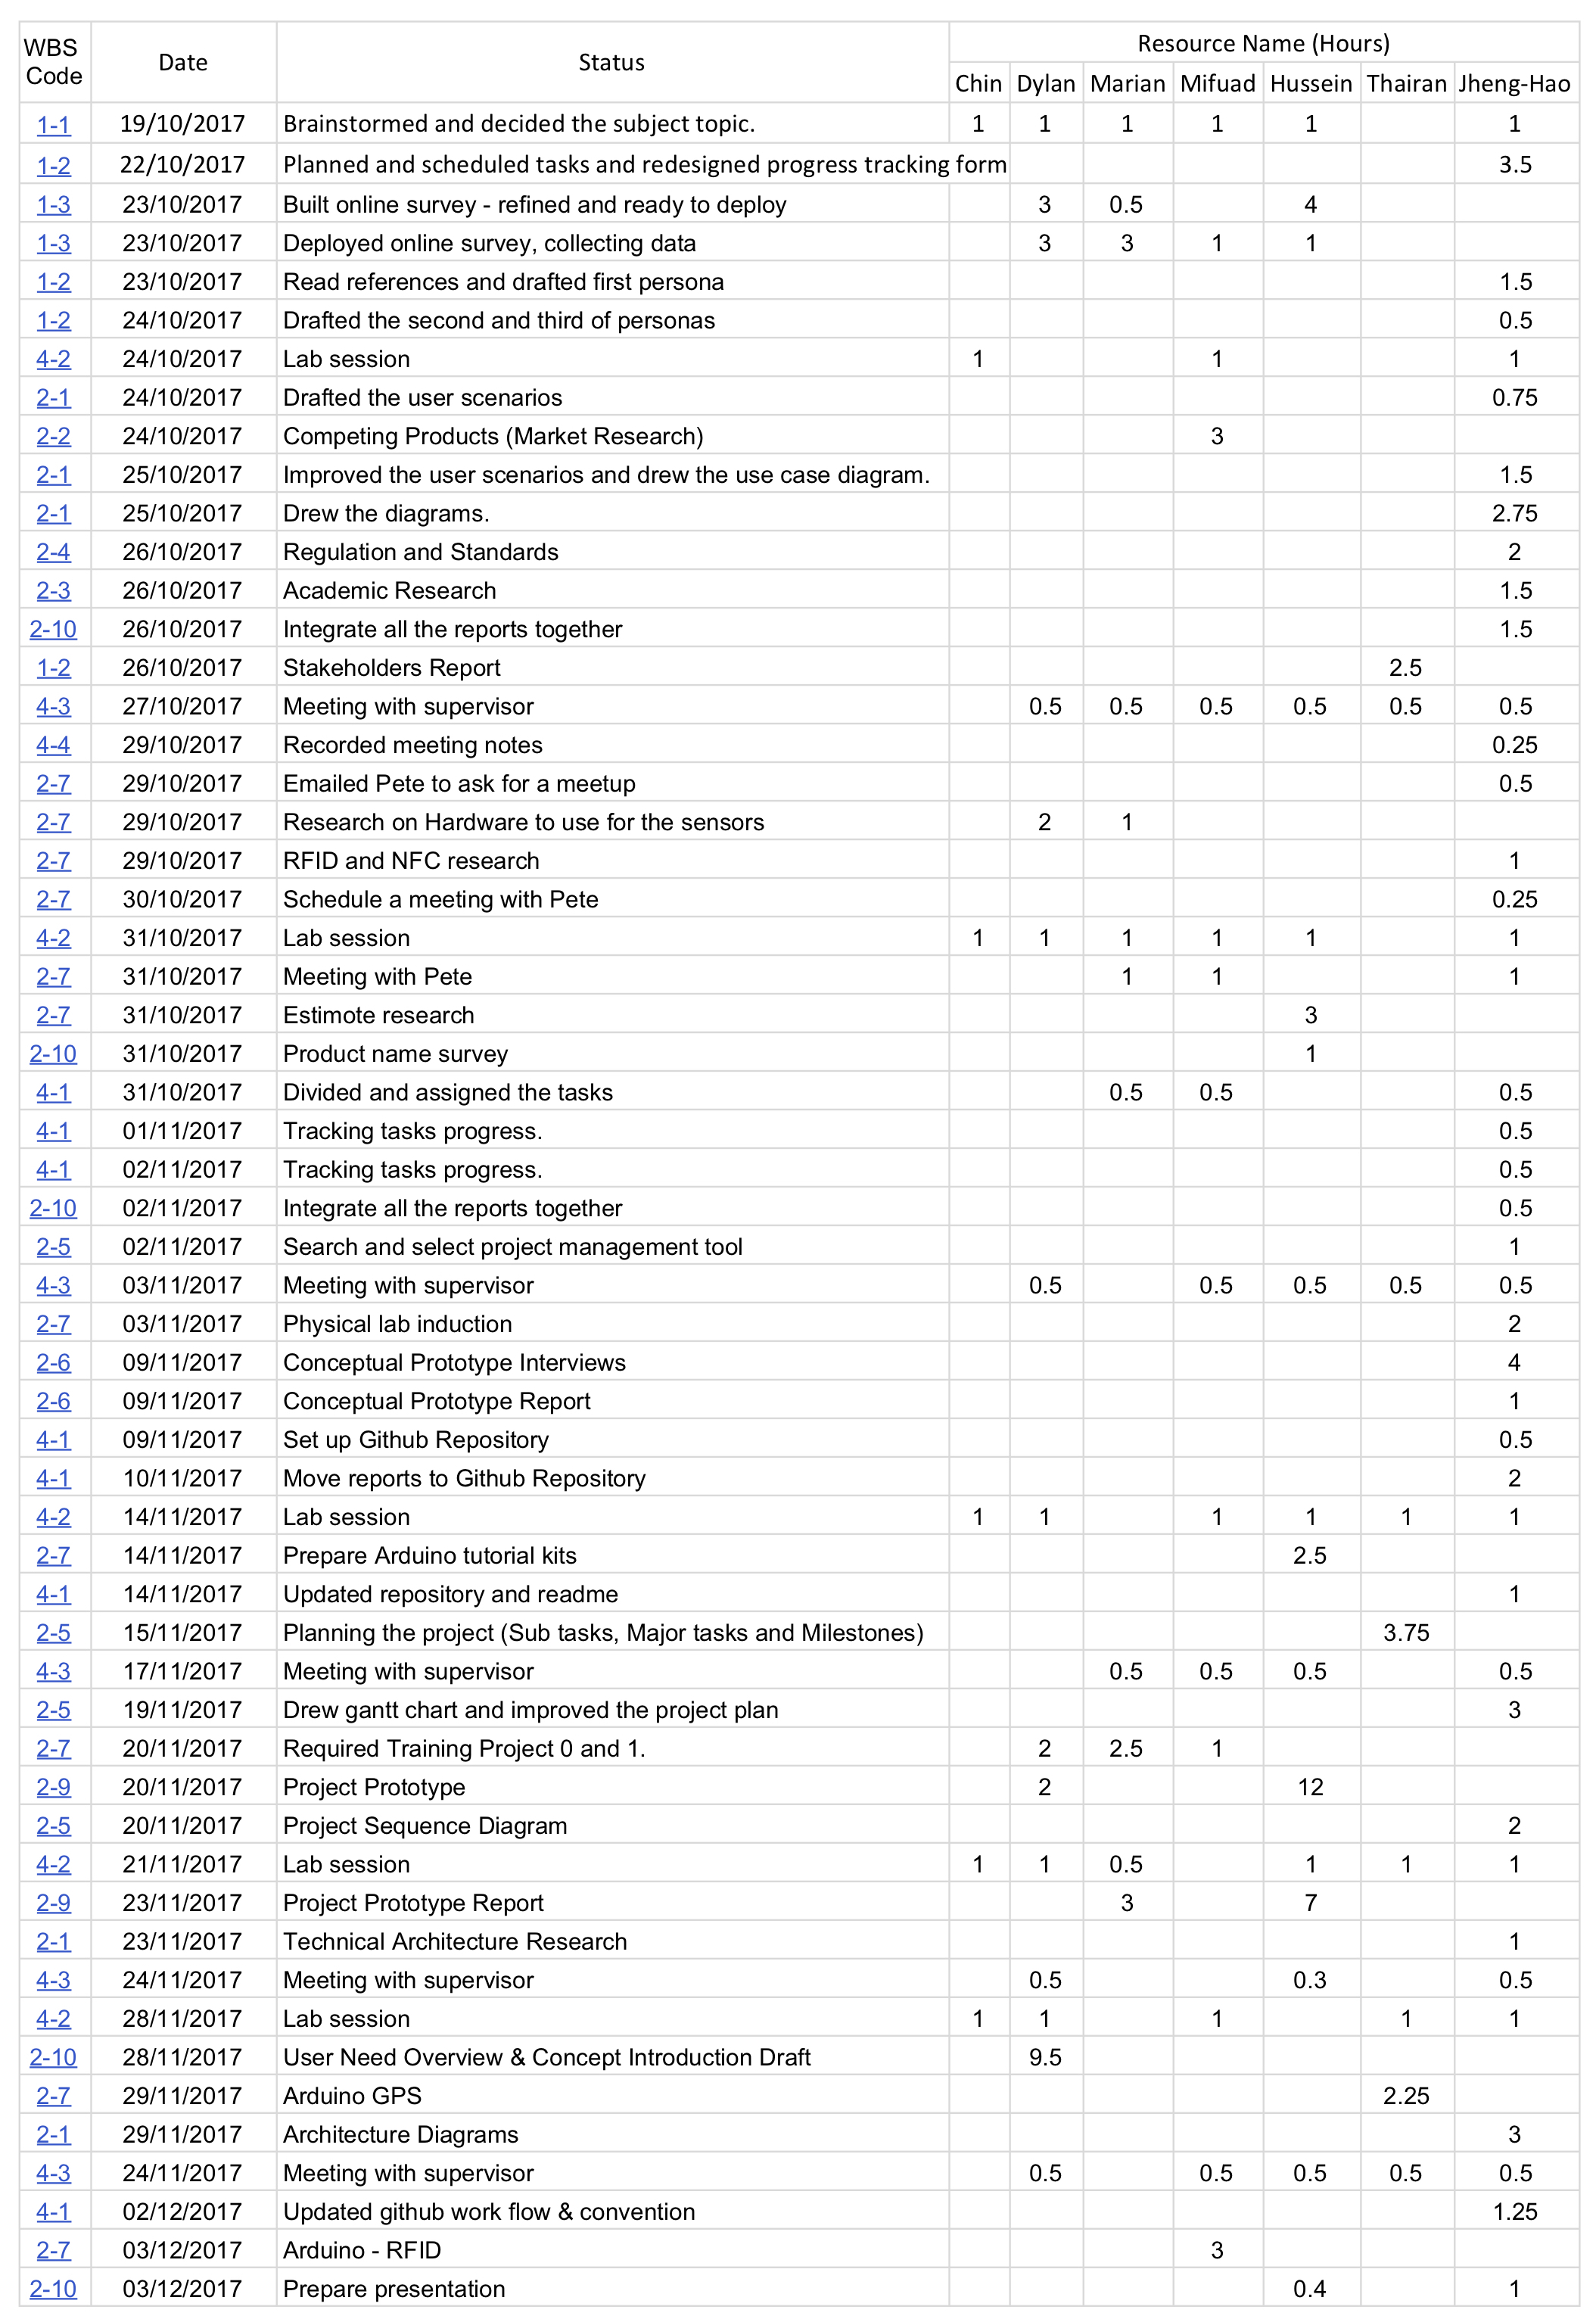
\includegraphics[width=.9\textwidth]{assets/12-9-3-progress-tracking-form-1.jpg}
        \caption{Progress Tracking Form-1}
        \label{fig:Progress Tracking Form-1}
      \end{figure}
      \begin{figure}[H]
        \centering
        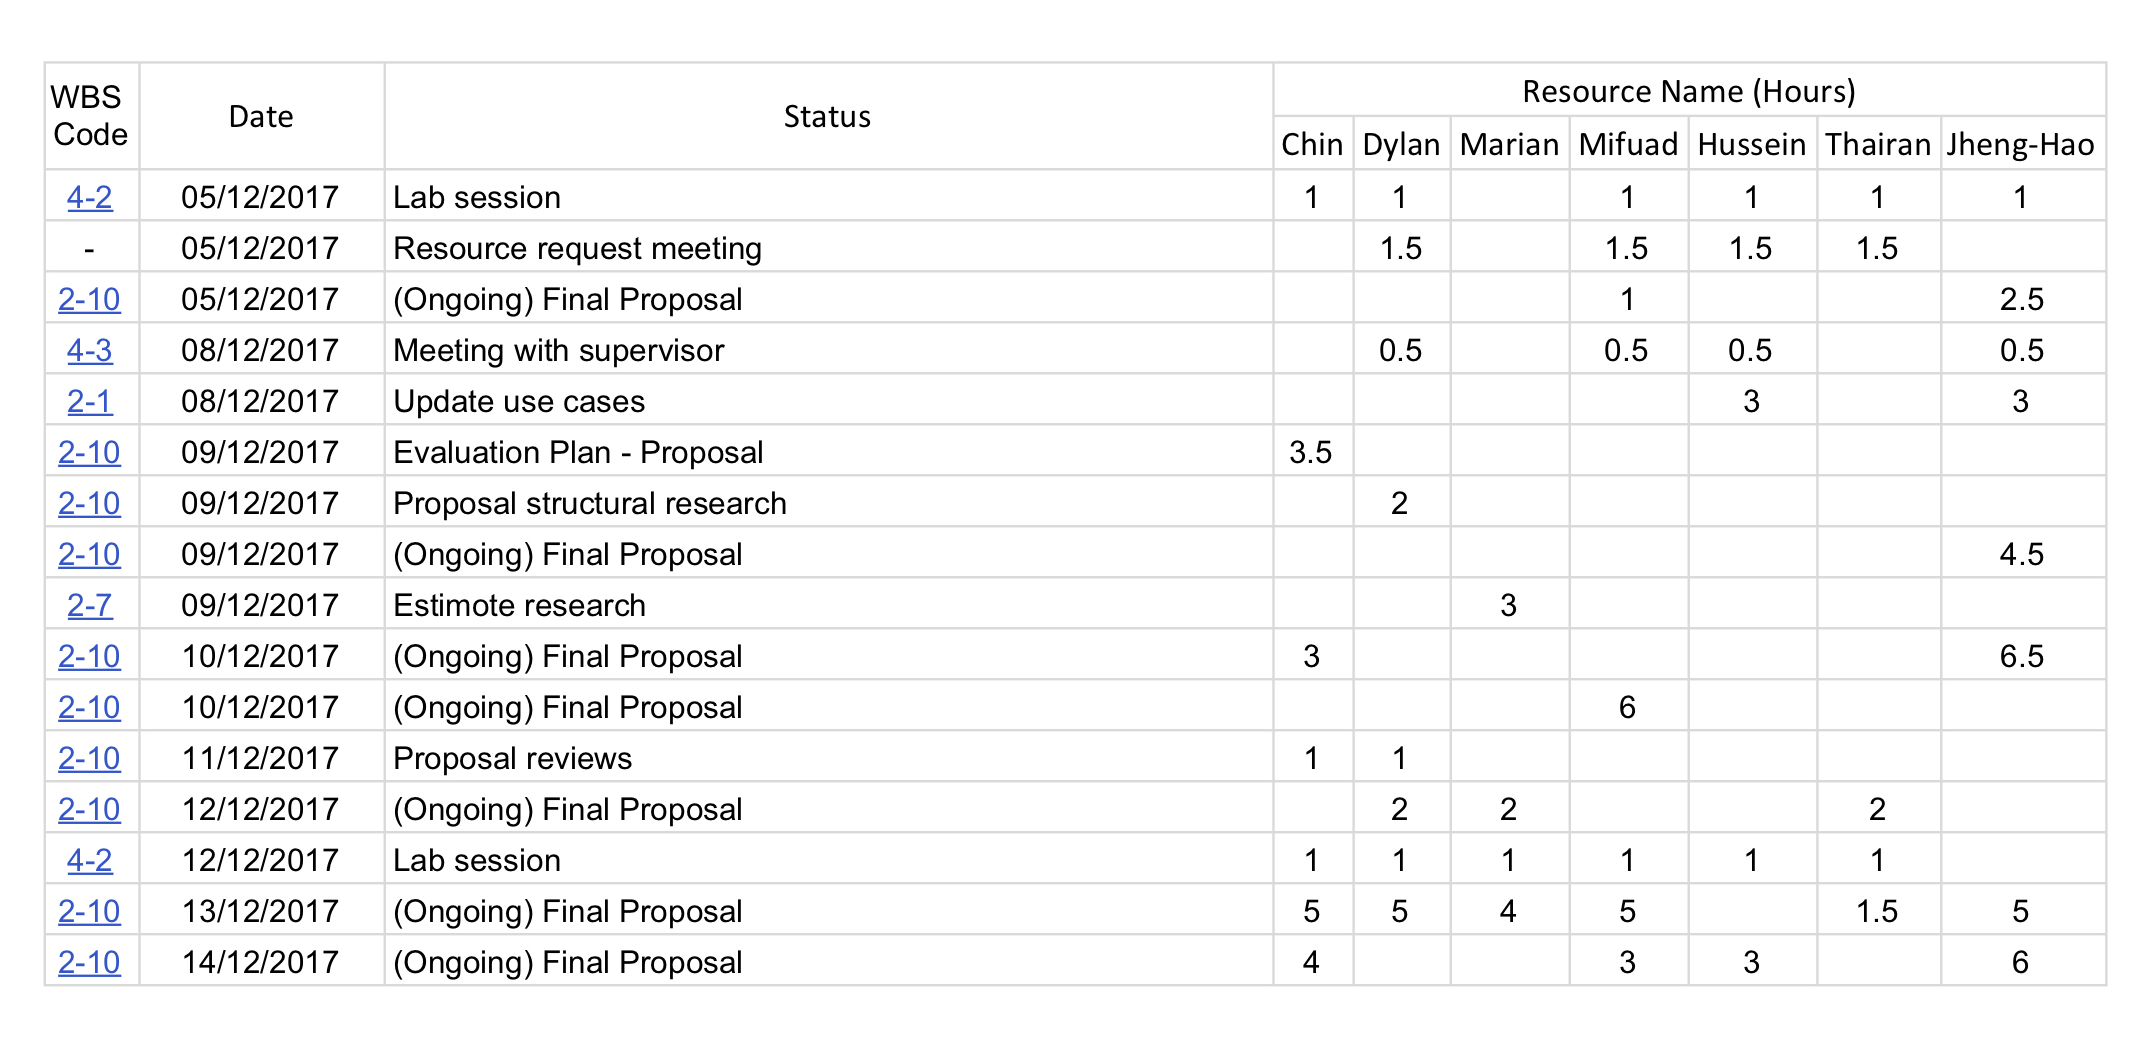
\includegraphics[width=.9\textwidth]{assets/12-9-3-progress-tracking-form-2.jpg}
        \caption{Progress Tracking Form-2}
        \label{fig:Progress Tracking Form-2}
      \end{figure}

      \begin{table}[H]
        \centering
        \resizebox{\textwidth}{!}{
          \begin{tabular}{ll}
            Label Name & Description \\
            \hline
            WBS Code & Work break down code, which indicates the category of the work for. \\
            Date & The working date. \\
            Status & The detail of the work. \\
            Resource Name(hour) & Usage of the resource(s) in hours. \\
            \hline
          \end{tabular}
        }
        \caption{Progress Tracking Form Label} 
      \end{table} 

    \section{Progress Tracking Charts}
      \label{appendix:progess-tracking-charts}
      \begin{figure}[H]
        \centering
        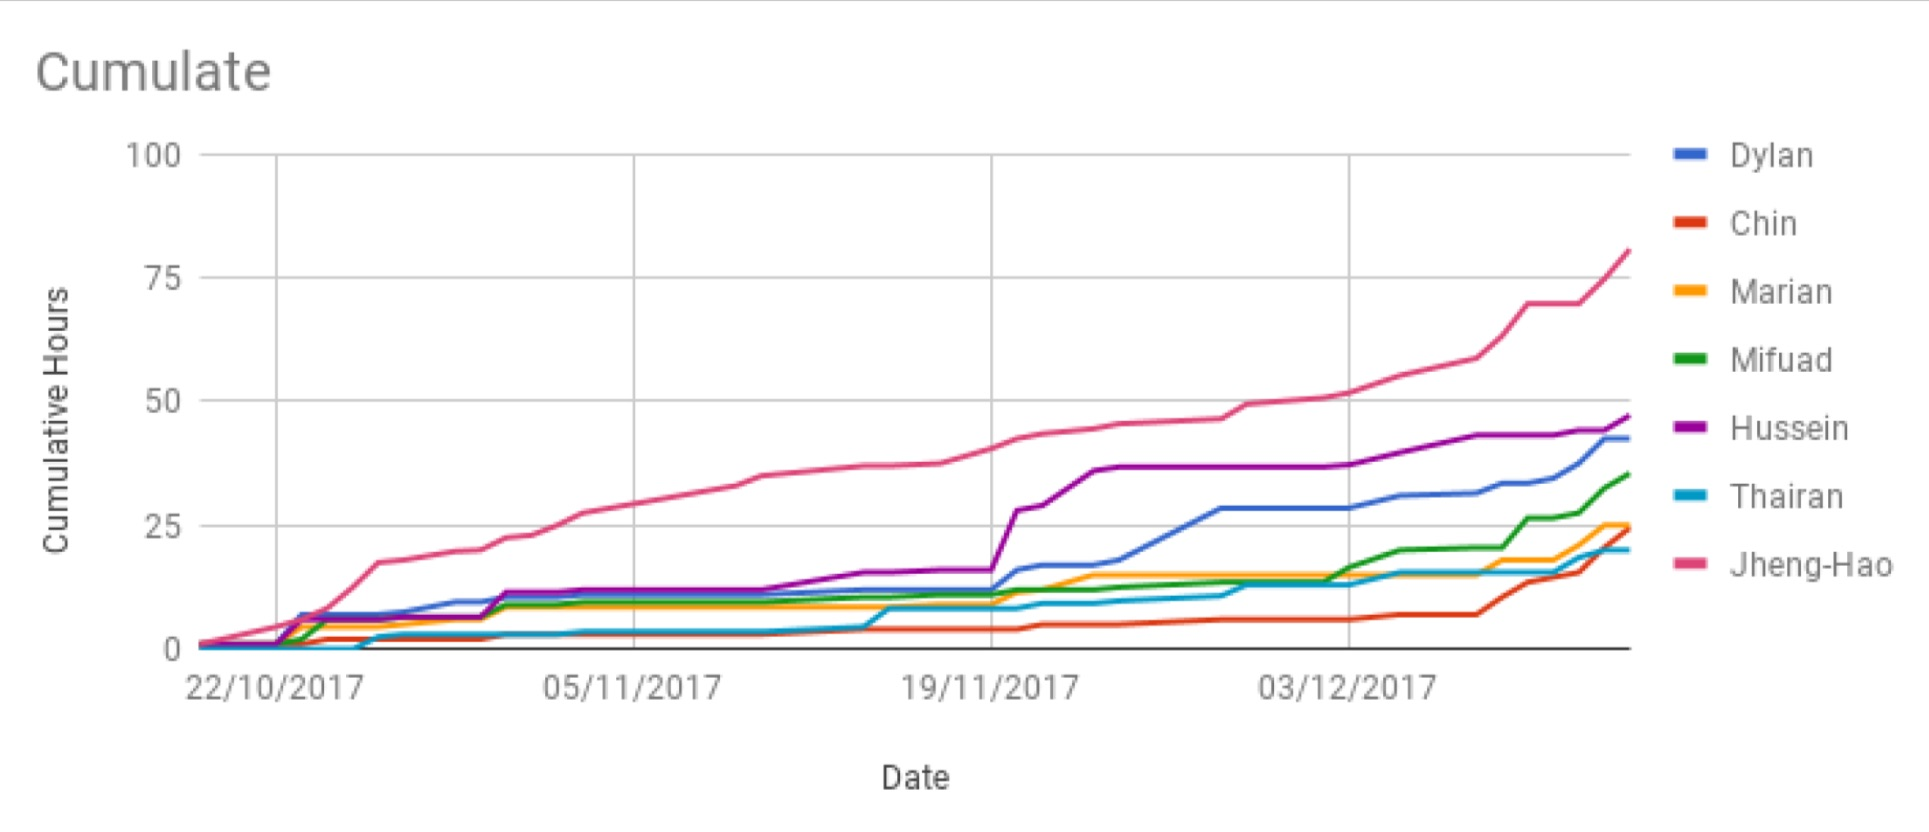
\includegraphics[width=1\textwidth]{assets/12-9-4-progress-tracking-chart-cumulate.jpg}
        \caption{Cumulate Line Chart}
        \label{fig:Cumulate Line Chart}
      \end{figure}

      \begin{figure}[H]
        \centering
        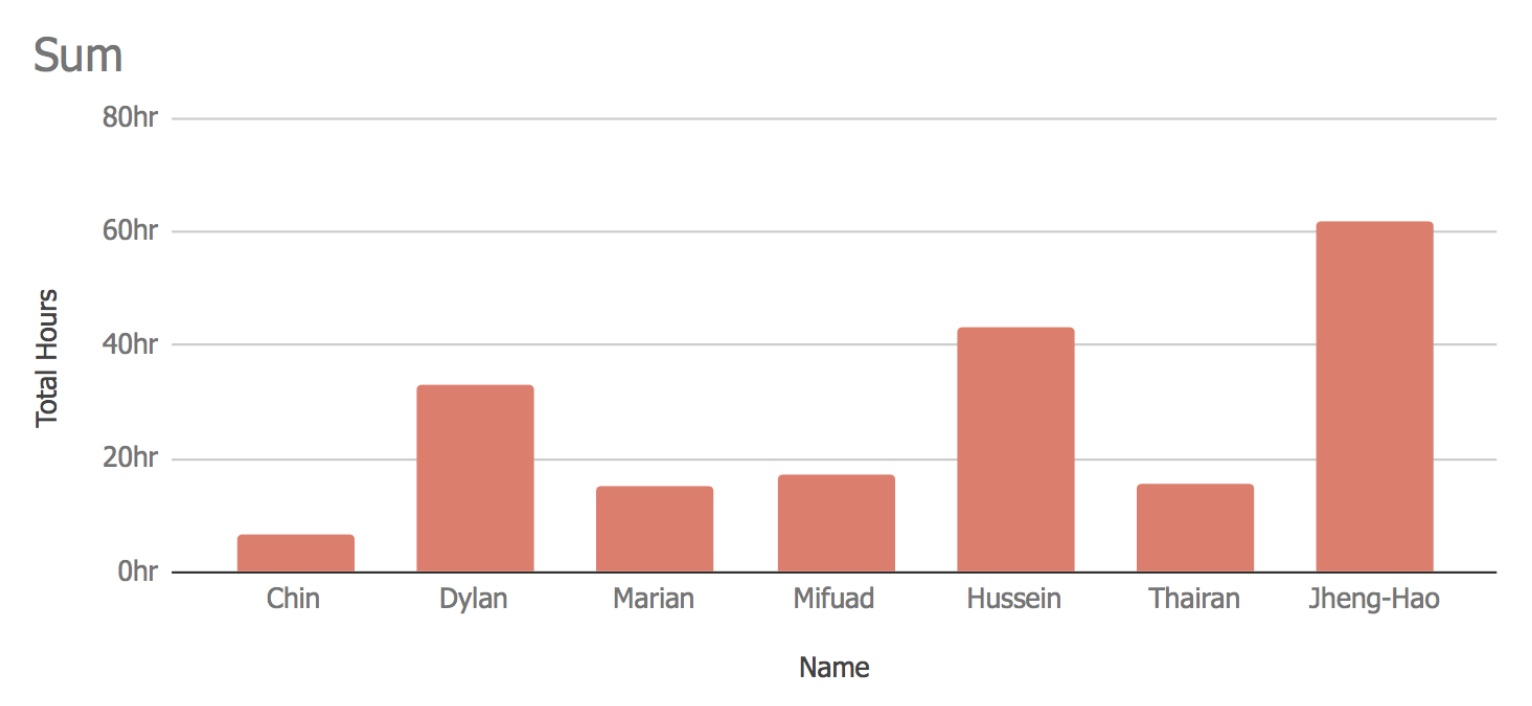
\includegraphics[width=1\textwidth]{assets/12-9-4-progress-tracking-chart-sum.jpg}
        \caption{Sum Line Chart}
        \label{fig:Sum Line Chart}
      \end{figure}

    \section{Project Management Tools Details}
     \label{appendix:project-management-tools-details}
     \begin{table}[H]
      \centering
      \resizebox{\textwidth}{!}{
        \begin{tabular}{ll}
          Platform & Usage\\
          \hline
          Slask & Inner communication.\\\hline
          Trello & Divides and assigns weekly tasks. (depreciated)\\
           & Records weekly meeting notes.\\\hline
          Google Sheets& Progress tracking form.\\
            & Gantt Chart.\\
            & Project Tasks List.\\\hline
          Github & Manage source code and report with fixed workflow.\\
           & Use issue feature to track developing progress.\\
           & Record weekly reports.\\
          \hline
        \end{tabular}
      }
      \caption{Project Management Tools Details} 
    \end{table} 

    \section{Github Directories}
      \label{appendix:github-directories}

      \lstset{language=Pascal}          % Set your language (you can change the language for each code-block optionally)
      
      \begin{verbatim}Write('Pascal keywords.');\end{verbatim}


      \begin{itemize}
      \item \begin{verbatim}/documents\end{verbatim}
        The reports for each week progress.
      \item \begin{verbatim}/proposal\end{verbatim}
        Paragraphs for each section of our first report
      \item \begin{verbatim}/src\end{verbatim}
        Software/hardwares source code.
      \item \begin{verbatim}/presentations\end{verbatim}
        Slides for the presentation in March.
      \item \begin{verbatim}/final-report\end{verbatim}
        Paragraphs for the final report.
      \end{itemize}


    \section{Github Workflow}
      \label{appendix: github-workflow}
      If you want to update any document or source code in the repository, please follow the {\bf workflow} and the {\bf naming convention} to maintain the consistency.
      
    \paragraph{tl:dr}
      \begin{enumerate}
        \item Issue
        \item Branch
        \item Work
        \item Commit
        \item Push \& pull request
      \end{enumerate}
      
      \paragraph{1. Issue}
      Before you start to work on either document or source code, make sure you browse the issue section to see if there is already an existing issue related to what you're going to work on. If you found one, than go to step 2-1.
      \paragraph{}
      If there is no such issue you're looking for, create a new one then. Condense the title and add more details in the description. Add the correct label to it and assignees as well.

      \paragraph{2-1. Check out the branch}
      Check out the corresponding branch on your local working space. If the issue you found is \#13, then the branch name should be like issue\-\#13\-xxxx. xxxx can be {\bf fix} or {\bf update}.
      \paragraph{2-2. Create a new branch based on that issue}
      If you can't find the issue about what you need to work on, create a new one on your own. Here is the naming convention:
      \paragraph{issue\-\#[ISSUE NUMBER]-[ACTION]}
      \begin{itemize}
        \item NUMBER: the number of the corresponding issue.
        \item ACTION:
        \begin{itemize}
          \item update: for report updating or feature updating, mainly for something continuously updating.
          \item fix: for fixing a bug or typo, mainly for something happen one time only.
        \end{itemize}
      \end{itemize}
      \paragraph{3. Work}
      As title, work on your branch and make sure you're on the right branch already. You can check it with \begin{verbatim}git branch\end{verbatim}
      \paragraph{4. Commit}
      To commit, here is the commit message:
      \begin{verbatim}
        [TYPE]: [SUBJECT LINE]
        [DESCRIPTION]
        [ACTION] #[ISSUE NUMBER]
      \end{verbatim}
    
      \begin{itemize}
        \item TYPE: Update or Fix. same as the ACTION on the branch name
          \begin{itemize}
            \item Update: for report updating or feature updating, mainly for something continuously updating.
            \item Fix: for fixing a bug or typo, mainly for something happen one time only.
          \end{itemize}
        \item SUBJECT LINE: briefly describe your changes.
        \item DESCRIPTION: describe the change in more details.
        \item ACTION:
        \begin{itemize}
          \item Close: to close of the branch and the issue forever (theoretically).
          \item Update: there should be future updating continuously.
        \end{itemize}
        \item ISSUE NUMBER: the issue number.
      \end{itemize}

      \paragraph{e.g. Update the report}
        \begin{verbatim}
          Update: Rewrite the project concept.
          Condense the project concept and add two new diagrams.
          Closes #1234
        \end{verbatim}
        
      \paragraph{e.g. Fix a bug}
        \begin{verbatim}
          Fix: Added missing header
          The app header was deleted accidently, added it back.
          Closes #12345
        \end{verbatim}
        Please review your change before every commit, which will massively reduce the possibility of finding bugs or typos after push the commit.
      
      \paragraph{5 Push \& pull request}
        After you push your commit, make a pull request on Github. Everyone can review your change and add comment. After reviewing I will either merge it to the master or ask you to do some change.  
    
      \subsection{Issue labels}
      Here are the categories of the issue labels, one issue can be assigned one or more labels.
        
        \begin{table}[H]
          \centering
          \resizebox{\textwidth}{!}{
            \begin{tabular}{ll}
              Label Name & Description\\
              \hline
              final report & related to final report\\
              enhancement & software functionality enhancement.\\
              bug & software bugs.\\
              hardware & hardware related.\\
              presentation & related to the presenation.\\
              project management & anything related to the project magement.\\
              proposal & related to the proposal content.\\
              weekly documents & weekly unsorted records.\\
              report & anything related to text, including final report, proposal and weekly documents.\\
              \hline
            \end{tabular}
          }
          \caption{Issue labels} 
        \end{table}      
    
    \section{Roles}
      \label{appendix: roles}
      \paragraph{Project Manager}
        \begin{enumerate}
          \item Members:
            \begin{enumerate}
              \item Jheng-Hao
              \item Hussein
            \end{enumerate}  
          \item Tasks:
          \begin{enumerate}
            \item Lead the discussion lab meeting and supervised meeting.
            \item Divide tasks.
            \item Monitor developing progress.
            \item Maintain workflow and Github repository.
          \end{enumerate}  
        \end{enumerate}
      
      \paragraph{Project Members}    
        \begin{enumerate}
          \item Members:
            \begin{enumerate}
              \item Muhammad
              \item Thairan
              \item Dylan
              \item Mahmudul
              \item Hussein
              \item Mariano
            \end{enumerate}  
          \item Tasks:
          \begin{enumerate}
            \item Contribute to overall project objectives.
            \item Complete individual task.
          \end{enumerate}  
        \end{enumerate}
    \end{appendices}

\end{document}
